\documentclass[conference]{IEEEtran}
\IEEEoverridecommandlockouts

\usepackage{cite}
\usepackage{amsmath,amssymb,amsfonts}
\numberwithin{figure}{subsection}
\usepackage{graphicx}
\usepackage{textcomp}
\usepackage{xcolor}
\usepackage[utf8]{inputenc}
\usepackage[labelfont=bf]{caption}
\captionsetup[table]{labelsep=space, 
         justification=raggedright, singlelinecheck=off, labelformat=empty}
\usepackage{kotex}
\usepackage{wrapfig} 
\usepackage{enumitem}
\usepackage{algorithm}
\usepackage{algpseudocode} 
\usepackage{hyperref}
\usepackage{listings}
\usepackage{cleveref, array, booktabs, threeparttable}
\lstset{
   breaklines=true,
   basicstyle=\ttfamily
   }
\def\BibTeX{{\rm B\kern-.05em{\sc i\kern-.025em b}\kern-.08em
    T\kern-.1667em\lower.7ex\hbox{E}\kern-.125emX}}





\begin{document}

\title{Smart Wine Cellar – Cave de Vin(Label D)\\ \LARGE DIOnyoS}

\author{\IEEEauthorblockN{Yujin Do}
\IEEEauthorblockA{\textit{College of Engineering}\\ 
\textit{Hanyang University}\\
\textit{Dept. of Information System}\\
Seoul, Korea\\
yujindo9@gmail.com}
\and
\IEEEauthorblockN{Yerin Cho}
\IEEEauthorblockA{\textit{College of Engineering}\\ 
\textit{Hanyang University}\\
\textit{Dept. of Information System}\\
Seoul, Korea\\
forjustice9839@gmail.com}
\and
\IEEEauthorblockN{Jungi Kim}
\IEEEauthorblockA{\textit{College of Engineering}\\ 
\textit{Hanyang University}\\
\textit{Dept. of Information System}\\
Seoul, Korea\\
damnum3@hanyang.ac.kr}
\and
\IEEEauthorblockN{Hyungseo Han}
\IEEEauthorblockA{\textit{College of Engineering}\\ 
\textit{Hanyang University}\\
\textit{Dept. of Information System}\\
Seoul, Korea\\
shorelinesquere@gmail.com}
}

\maketitle
\thispagestyle{empty}
\pagestyle{empty}
\begin{abstract}
Our team is trying to develop User-Friendly wine cellar by appending additional functions to “LG wine cellar". By capturing and registering wines in "Cave de Vin(label D)", users can effectively manage their wines and wine cellar. Using wine recommendation and purchasing function can promote additional consumptions to wine and wine cellar. Also, by sharing the scene that enjoying wine on the social media, people can enjoy the marketing effect of LG wine cellar.
\end{abstract}



\begin{table}[h]
\caption{Role Assignments}
\def\arraystretch{1.24} \small

\begin{tabular}{|p{1.8cm}|p{1.4cm}|p{4.4cm}|}

\hline
Roles & Name & Task description and etc. \\ \hline
Quality\par Assurance Manager&  Hyungseo Han & They understand demand and requirement of application. They test the overall application from customers’ point of view and report error and bug. They strive to maximize user experience by considering UI / UX. \\ \hline

Software \par Developer & Yerin Cho \par Jungi Kim  & Software developers think about the software in general. They design and implement the requirements of application. They also strive to satisfy users and customers. \\ \hline

Development \par manager & Yujin Do & Development manager manages the overall project. They strive to meet the needs of customers. They collect the feedback from users. After collecting feedback, they advise software developers to improve application quality. \\ \hline

\end{tabular}

\end{table}
\section{Introduction} \noindent\textit{Motivation}\\
\indent Due to the COVID-19, the number of people who drink at home has increased significantly. Wine is one of the most popular drinks for people who drink alone, and wine imports rose 110\% year-on-year in the first half of last year. Thus, the demand for wine cellars also increased. However, there are too much information to enjoy wine, such as the way to store wine, or detailed information of the wines. But services that support people who try to get information of in the wine in Korea are poor. Therefore, our team felt the needs for a service that effectively records and manages the wine that I drink and drank, and further recommends and induces to user to purchase the wine.\\



\noindent\textit{Problem Statement}\\
\indent There are many wine applications such as Vivino. However, there is a limitation that the service is based in a foreign country other than Korea. Currently, it is difficult to find information to better enjoy wine in Korea. Accordingly, the necessity of providing various wine information, wine purchase service, SNS sharing service, etc. to enjoy wine better by linking with the wine cellar to facilitate humidity and temperature control was recognized.\\ 
  
  
  
\noindent\textit{Solution}
\begin{enumerate}
\item Available to manage wine and wine cellar effectively. 
- It is possible to manage users' wines and wine cellar in one
application.

- Effective wine management is possible by recommending
appropriate wine storage methods to users.

- Once the wine is registered, detailed information can be
easily offered.

\item Available to create additional consumption of wine cellar. 
- By recommending new wines based on registered wines,
new wines can be made, and even wine cellars can be
consumed. B2B business development through collaboration
with wine sellers is also possible.

- By providing a user-friendly SNS sharing service, the
promotional effect of LG Wine Cellar can also be expected.\\
\end{enumerate}


\noindent \textit{Research on Related Software}
\subsection{Vivino}
Vivino is the world’s largest wine application, which helps users discover the perfect wine. When users scan wine label, it shows ratings, reviews, and prices of the wine. Users can easily click to purchase bottles on web or mobile in application. And it keeps track of wines which users like and recommend other wine for user.
  
\subsection{My Own Refrigerator (from GS25 convenience store)}
My Own Refrigerator is a convenience store shopping service that allows user to discount, earn, pay directly from mobile. And user can store products purchased at the store. One of key features is ‘Storage Box’. Users can check the storage history of purchased products and can use them later.

\subsection{CellWine}
CellWine is an application which provides mobile wine collection. When users scan wine labels, application keeps track of cellars and log the cost and quantity of collections anytime, anywhere. And it helps users to record own rating score and flavors. It also helps users to explore different wine by giving recommendations. 

\subsection{ThinQ}
ThinQ is an application which connects washer, air conditioner, TV and other LG appliances and mobile phones. It automatically accesses the current state of products and get immediate notifications of products. Existing LG wine cellar only supports few functions. Users can control temperature of wine upper, wine lower and fridge drawer by ThinQ. And if users say, ‘Hi LG, open the refrigerator door’, or put your foot close to the product, the door open automatically.

\section{Requirements}
\subsection {\textbf{Wine cellar registration screen}}
\begin{enumerate}
\item Select the LG wine cellar that the customer purchased.
\item Enter and register the serial number of the purchased product.
\item After authenticating the information (serial number, model), the application automatically creates the shape of wine cellar that user purchased and an empty floor of wine cellar.
\end{enumerate}
\subsection {\textbf{Wine cellar screen - default screen after registered model}}
\begin{enumerate}
\item Floors management menu

\begin{enumerate}
\item Wine add – on
 \begin{enumerate}
    \item Customers take a photograph of the label of the wine
    \item The application analyzes the label that from user-taken
	photograph.
	\begin{enumerate}
	\item Application analyzes wine name, and date of 
    manufacture.
    \item Customers enter the purchase date.
    \item Application shows information related to the 
    registered wine - tasting notes, average price, country,
    grape variety, food pairing, winery, vintage,
    comparison, management method, recommended
    glass, etc.
	\end{enumerate}
	\item After judging whether the temperature and humidity of the floor selected by the user is suitable, the application
can recommend another floor
\end{enumerate}

\item Temperature, Humidity management of each floor of model
\begin{enumerate}
    \item Inside the app, the temperature of each floor and the humidity of the model can be monitored on the left or right side of the virtual model.
    \item If the customers want to adjust the temperature and 	humidity, then customers can modify these by pressing 	the mark in the application.
\end{enumerate}

\item Wine cellar lock function
\begin{enumerate}
    \item Customers can activate lock function to full floor or 	floor by-floor via application.
    \item To prevent theft and damage to wine cellar, customers 	can set alarms on locked floors.
\end{enumerate}
\end{enumerate}

\item Individual wine screen
\begin{enumerate}
\item Detailed information about selected wine
\begin{enumerate}
    \item Customers choose one of the wines in their own wine
    cellar model.
    \item The application displays detailed information about 	the selected wine, such as manufacture date, expiration 	date, purchase date, alcohol percentage, etc.
    \item When customers drink a bottle of wine, user can delete the wine from wine cellar by clicking 'empty?' button.
\end{enumerate}
\end{enumerate}
\item Wine history screen
\begin{enumerate}
\item Show the whole of wines that customer has drank so far.
\begin{enumerate}
    \item Display the drank wines using wine corks.
    \item Recommends of wines that are likely to suit
	customers’ taste based on the history of wine customers	have drunk.
	\item Recommendations are based on price, grape variety,  
   	taste and smell, and customers’ nationality.
\end{enumerate}
\end{enumerate}
\end{enumerate}

\subsection{\textbf{Social media quick link function}}
\begin{enumerate}
    \item This function helps user to share wine and wine cellar which he
has on social media such as ‘Instagram’, ‘Twitter’, ‘Facebook’
and so on.

\item Auto complete hashtag


When user uses ‘social media quick link’, user can get ‘auto
complete hashtag’ function. Hashtag is made based on the
name of wine cellar, and the name, type, taste of the wine,
which helps users upload the post easily on social media.
\item Share my Wine Cellar

  User can share the image of wine cellar. By capturing the
image of virtual wine cellar, user can save the image into jpg
file format or share it on social media.

\item Share my Wine History

\begin{enumerate}
    \item User can share ‘my wine history’
    \item The wine he has drunk can be shown into the cork icon.
The more he drinks wine, the more cork stamps will be
collected.
    \item The price of wine is shown in the image of receipt, which
shows each name of wines and each price and total price.
\end{enumerate}

\item Make my Wine Topster

User can make ‘wine topster’, which means collage of
favorite wine.
\begin{enumerate}
    \item First, user sets the layout of topster. User can set the
rows, columns (n*n) and background image of collage.
\item Second, user makes the collage based on the images
of wine label which were saved in application before.
\item Third, user can download wine topster into jpg/png
file format or can share it on social media directly.
\end{enumerate}
\end{enumerate}

\subsection {\textbf{Wine Recommendation function}}

\begin{enumerate}
\item Wine promotion nearby to me 


When there are discounts on wine near to user, application gives push alarm to user. It helps user to make a reservation or to buy wine at reasonable price.
\item Wine Reservation


If user is looking for rare wine, user can register wine alarm which relates to wine shop. When wine is stocked, alarm goes off and lets user know that wine is available to buy. Then user can make a reservation or buy wine.
\item Calendar Sync


When user synchronizes google calendar with application, it recommends wine which fits in with schedule. Recommendation can be made based on wine which user already has. If there isn't any suitable wine, application recommends user to purchase wine from wine shop nearby.
\end{enumerate}

\section{Development Environment}
\subsection{Choice of software development platform}
Our team will develop application in the environment of Mac operating system. Also, our application will run on the Android OS environment. Android OS is a mobile operating system based on the Linux kernel made by Google, and it is the operating system that most smartphone manufacturers choose except for Apple. As you can see from the charts below,72\%of people around the world use Android-equipped smartphones, and 73\%of people in Korea also use Android OS. The reason for this high market share is that the SDK (Software Development Kit) for developing Android applications and the related Kernel are open for free, so many people have been able to develop various applications without restraint. However, since the share of IOS made by Apple is over 20\%, we'll use the React-Native framework that can develop Android and IOS applications simultaneously. As a result, it'll make it easier to develop iOS applications in the future. Therefore, our team will use Android Studio to create applications based on the Android platform, and usage of the languages will be React-Native, Java Spring, and MariaDB.
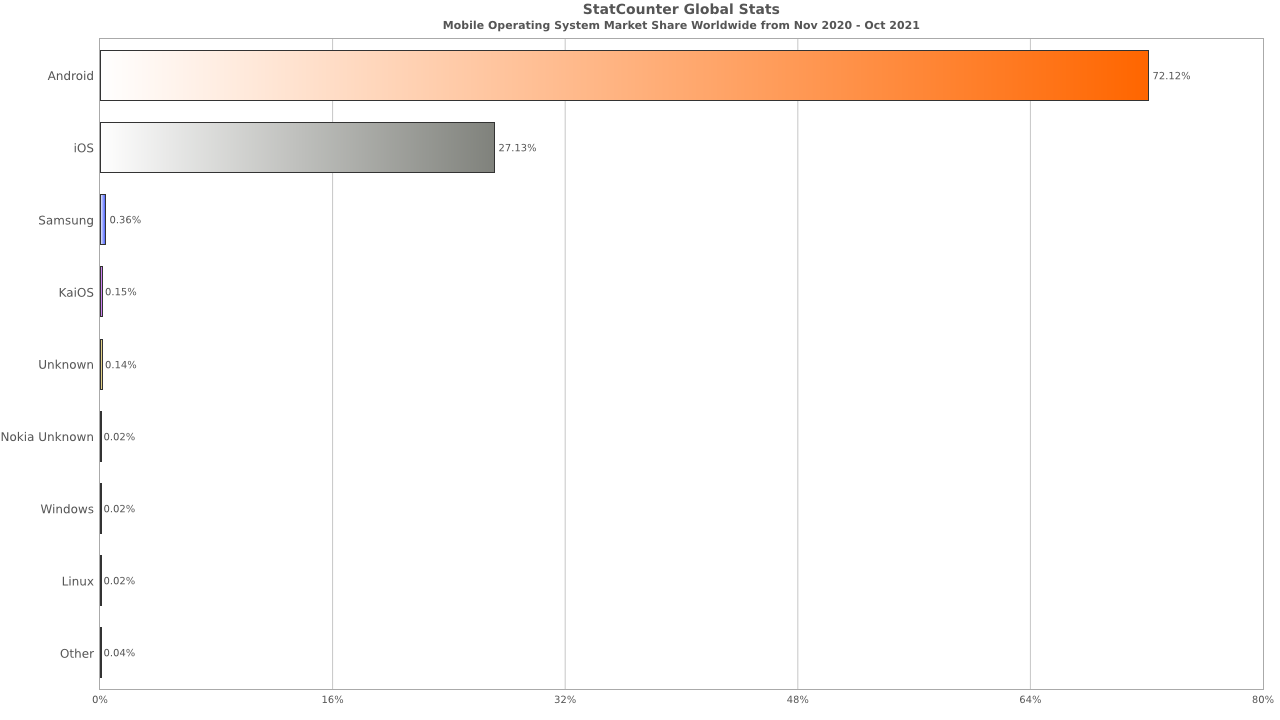
\includegraphics[width=10cm]{globalstats1.png}
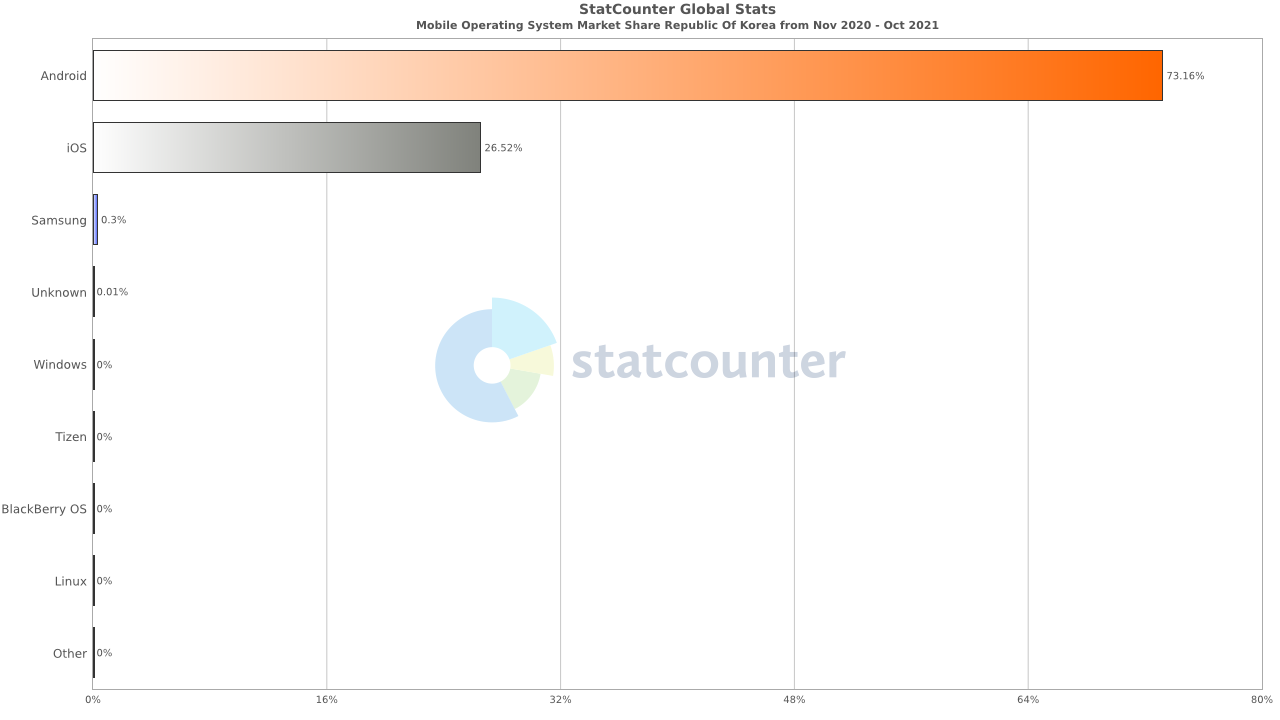
\includegraphics[width=10cm]{globalstats2.png}

\begin{enumerate}
    \item React-Native
    
    
    React Native is an open source mobile application framework developed by Facebook. It is used to develop applications for Android, iOS, Web, and UWP, allowing developers to use React in addition to native platform features. React Native has the biggest advantage of being able to create native UI for Android and iOS using JavaScript, and create high-quality UI faster than using XML/Java/Kotlin. In addition, we can quickly check changes or modifications with our eyes, making QA or feedback easier to proceed. 
    \item Spring - JAVA Framework
    
    
    The Spring Framework is an open source application framework for the Java platform. It is used as a foundation technology for the e-government standard framework recommended for use in the development of web services by public institutions in Korea.
    \item MariaDB
    
    
    It is necessary to store and manage information about wine cellars, users of wine cellars, wine stored in wine cellars. For this, MariaDB is used. MariaDB is an open-source relational database management system (RDBMS). It is based on the same source code as for MySQL and follows the GPL v2 license. It also supports the latest SQL functions such as common table expressions (CTE), window functions, temporary data tables, and JSON functions.
\end{enumerate}
\subsection{Software in use}
There are already two existing popular apps that manage and record purchased wine. Vivino was launched in 2010 and has recorded more than 50 million downloads so far and maintains a 4.6 rating in the Google Play Store. As it has been a long time since it was released, it has many users' evaluations and reviews. Cellwine was launched in 2016, recording more than 50,000 downloads, and has a rating of 4.0 points in the Play Store. Both Vivino and CellWine can register wine by taking wine labels and record wine that users have been drinking so far. And users can search for a variety of wines around the world, check the ratings and information of each wine, reviews from other tasters, prices, and recommended foods that goes well with wine. And based on the wines that have been drunk and recorded so far, those two apps also recommend new wines that suit the user. Vivino also has the function to purchase wine from the application.
\subsection{Task Distribution}
\begin{table}[H]
\begin{center}
\begin{tabular}{|c|c|}
\hline
Name & Task\\
\hline
 Cho Yerin & App backend\\
 \hline
Do Yujin & App frontend, UI/UX\\
\hline
Han Hyeongseo &bApp backend, App frontend\\
\hline
Kim Jungi & App frontend, Infra\\
\hline
\end{tabular}
\end{center}
\end{table}

\section{Specification}
\subsection{Welcome Page}
\centerline{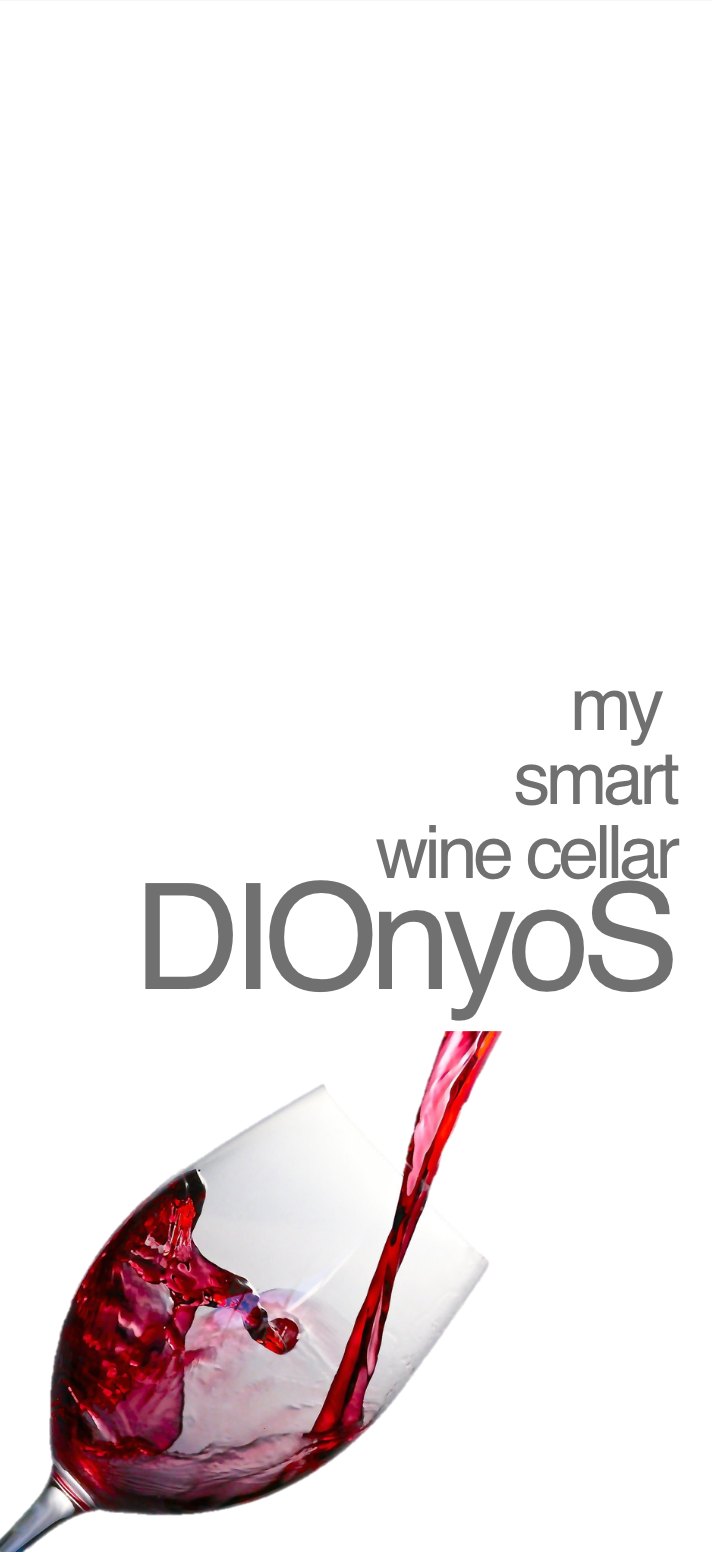
\includegraphics[width=5cm]{firstpage.png}}
\centerline{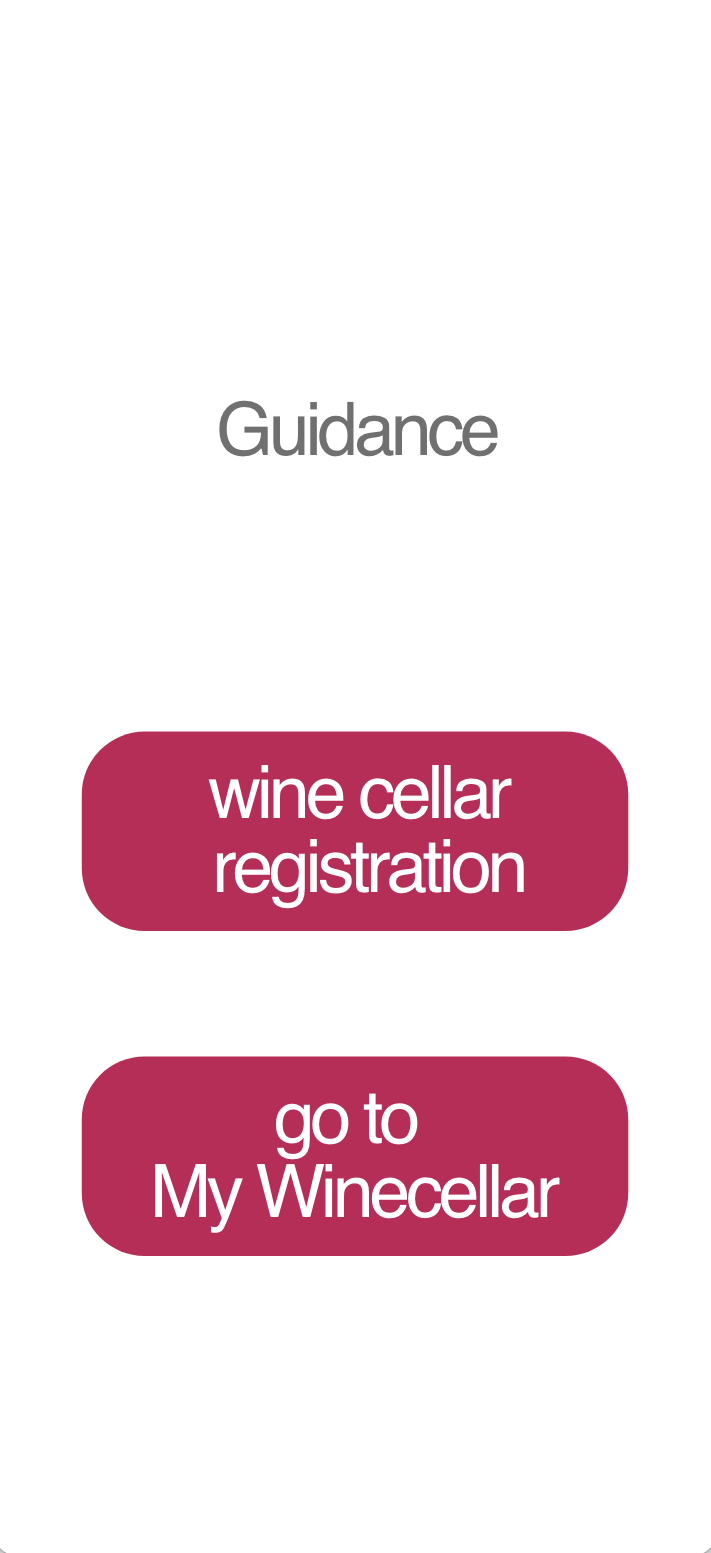
\includegraphics[width=5cm]{guidance.png}}
Welcome page is the first screen when downloading this application. If user runs the application, welcome page, which is consisted of ‘Wine cellar registration’ button and ‘go to My Wine cellar’ button.
\begin{enumerate}
\item \textit{\textbf{Wine cellar registration}}\\
\centerline{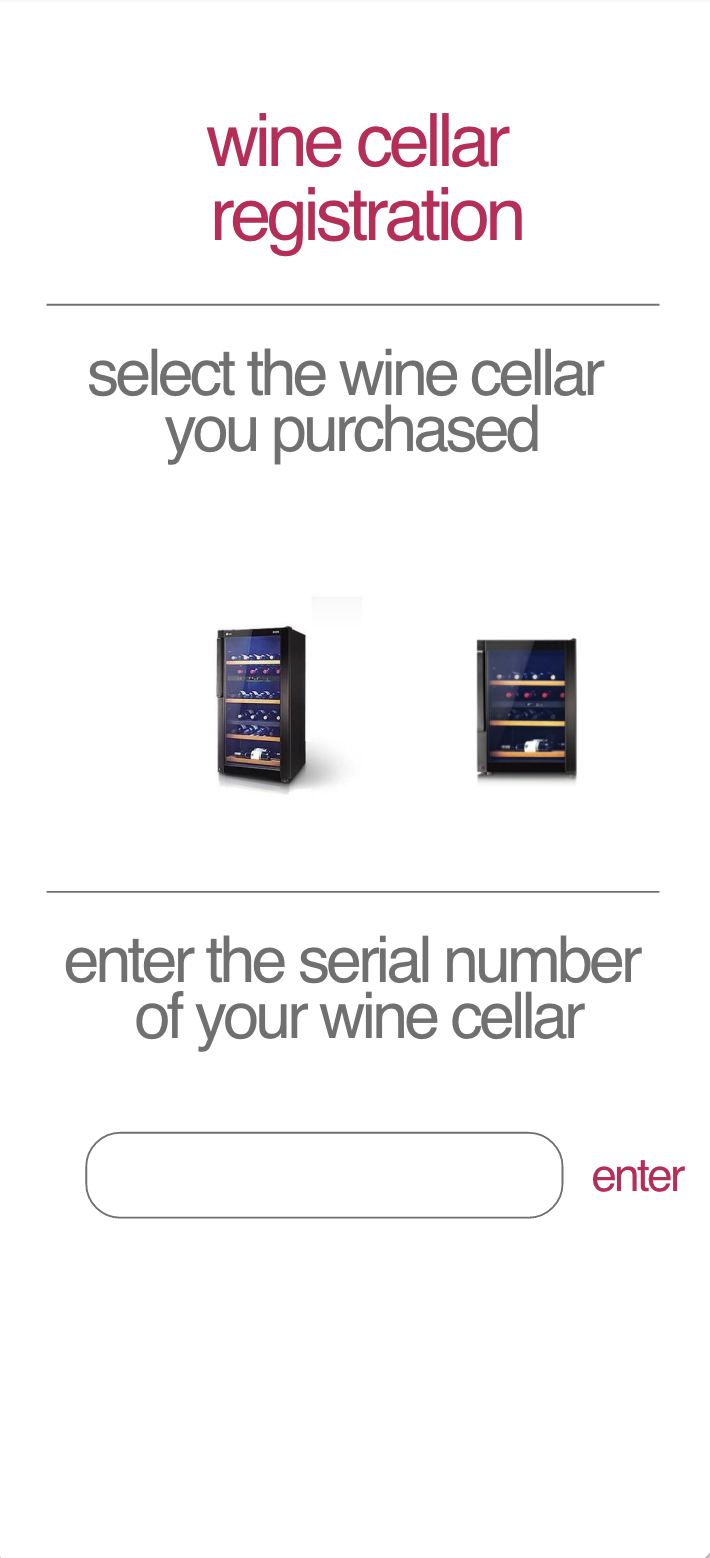
\includegraphics[width=5cm]{winecellarregi.png}}
Wine cellar registration button is for user who is first in ‘DIOnyoS’ application and who wants to register another wine cellar in ‘DIOnyoS’. When user press this button, user has to select the wine cellar which he purchased from horizontal scroll. And then user has to enter the serial number of the wine cellar.\\
\centerline{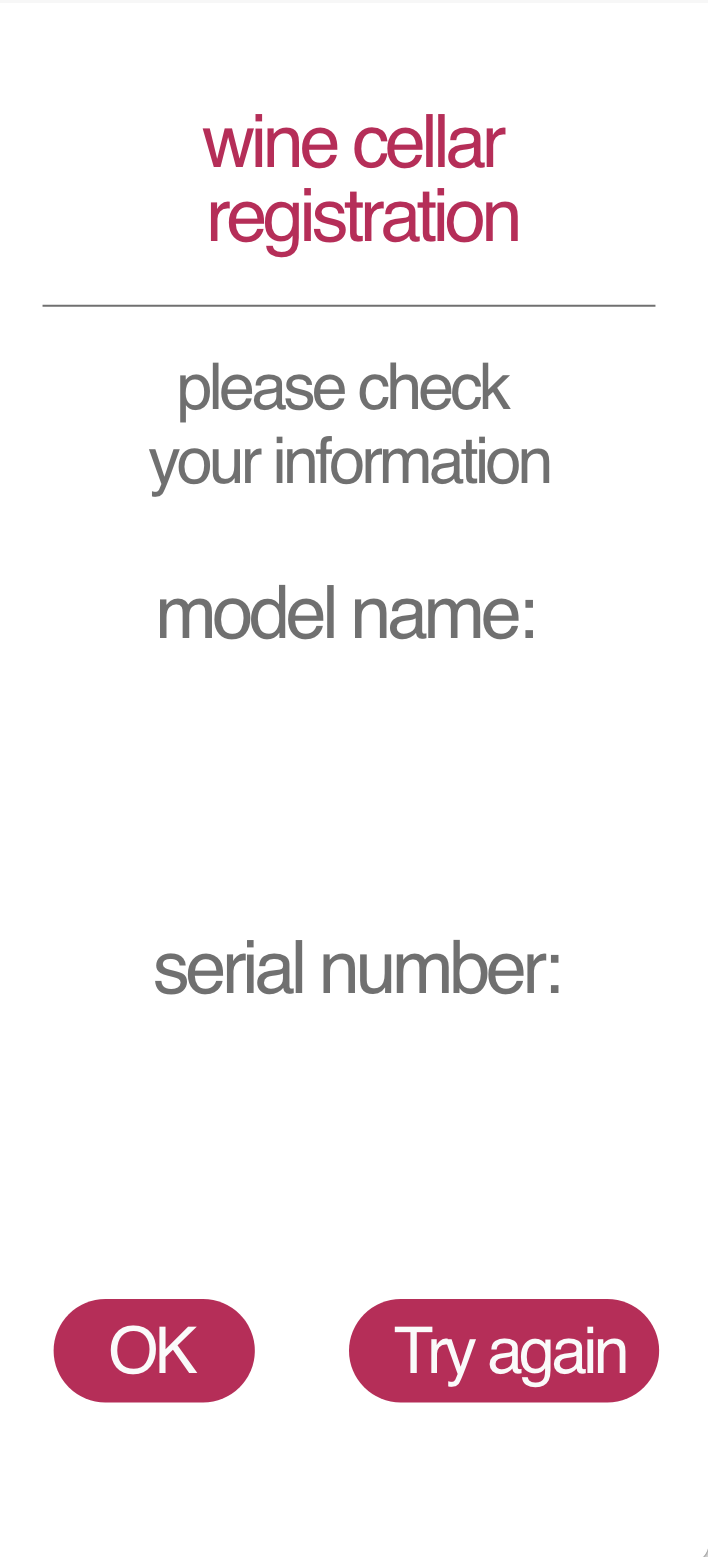
\includegraphics[width=5cm]{regicheck.png}}
After user ends two steps for wine cellar registration, there will be a page for check. If there isn’t any error in registered information, user will push ‘ok’ button to go to ‘My Wine cellar’, which is main page. Or else, user will push ‘try again’ button to re-enter information for wine cellar registration.
\item \textit{\textbf{Go to my Wine cellar}}\\
If user presses this button, user can go to ‘My Wine cellar’, which is main page of application.
\end{enumerate}

\subsection{My Wine cellar (Main page)}
\centerline{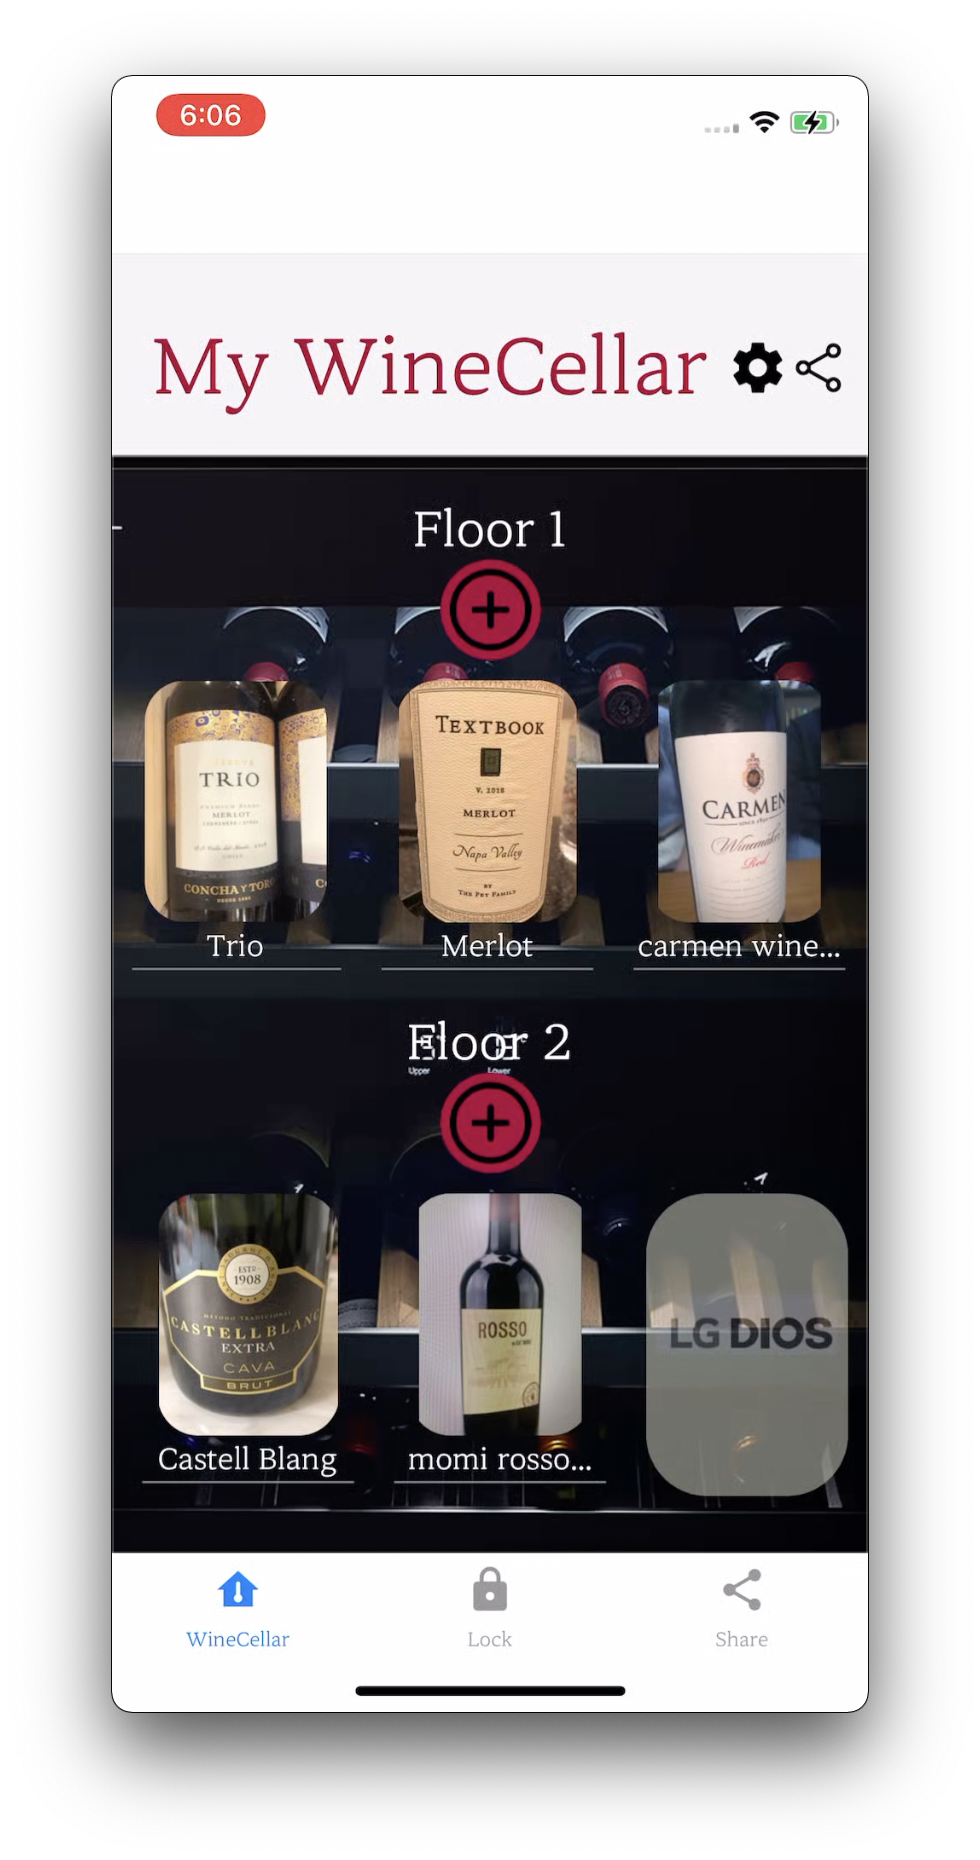
\includegraphics[width=5cm]{mywinece.png}}
My Wine cellar is the main page of application. My Wine cellar is virtual wine cellar, which shows image of registered wine label in application. Wine cellar is consisted of 4 floors. As there is difference in the size of wine cellar, main page lets user to see wine by scrolling rows.

\begin{enumerate}
    \item \textit{Navigation bar}\\
    Navigation bar is consisted of 4 icons, plus, lock, alarm and share.
    
    \begin{enumerate}
        \item \textit{\textbf{Wine registration} (Plus icon)}\\  
        When user presses Plus icon, user starts wine registration step.
        \centerline{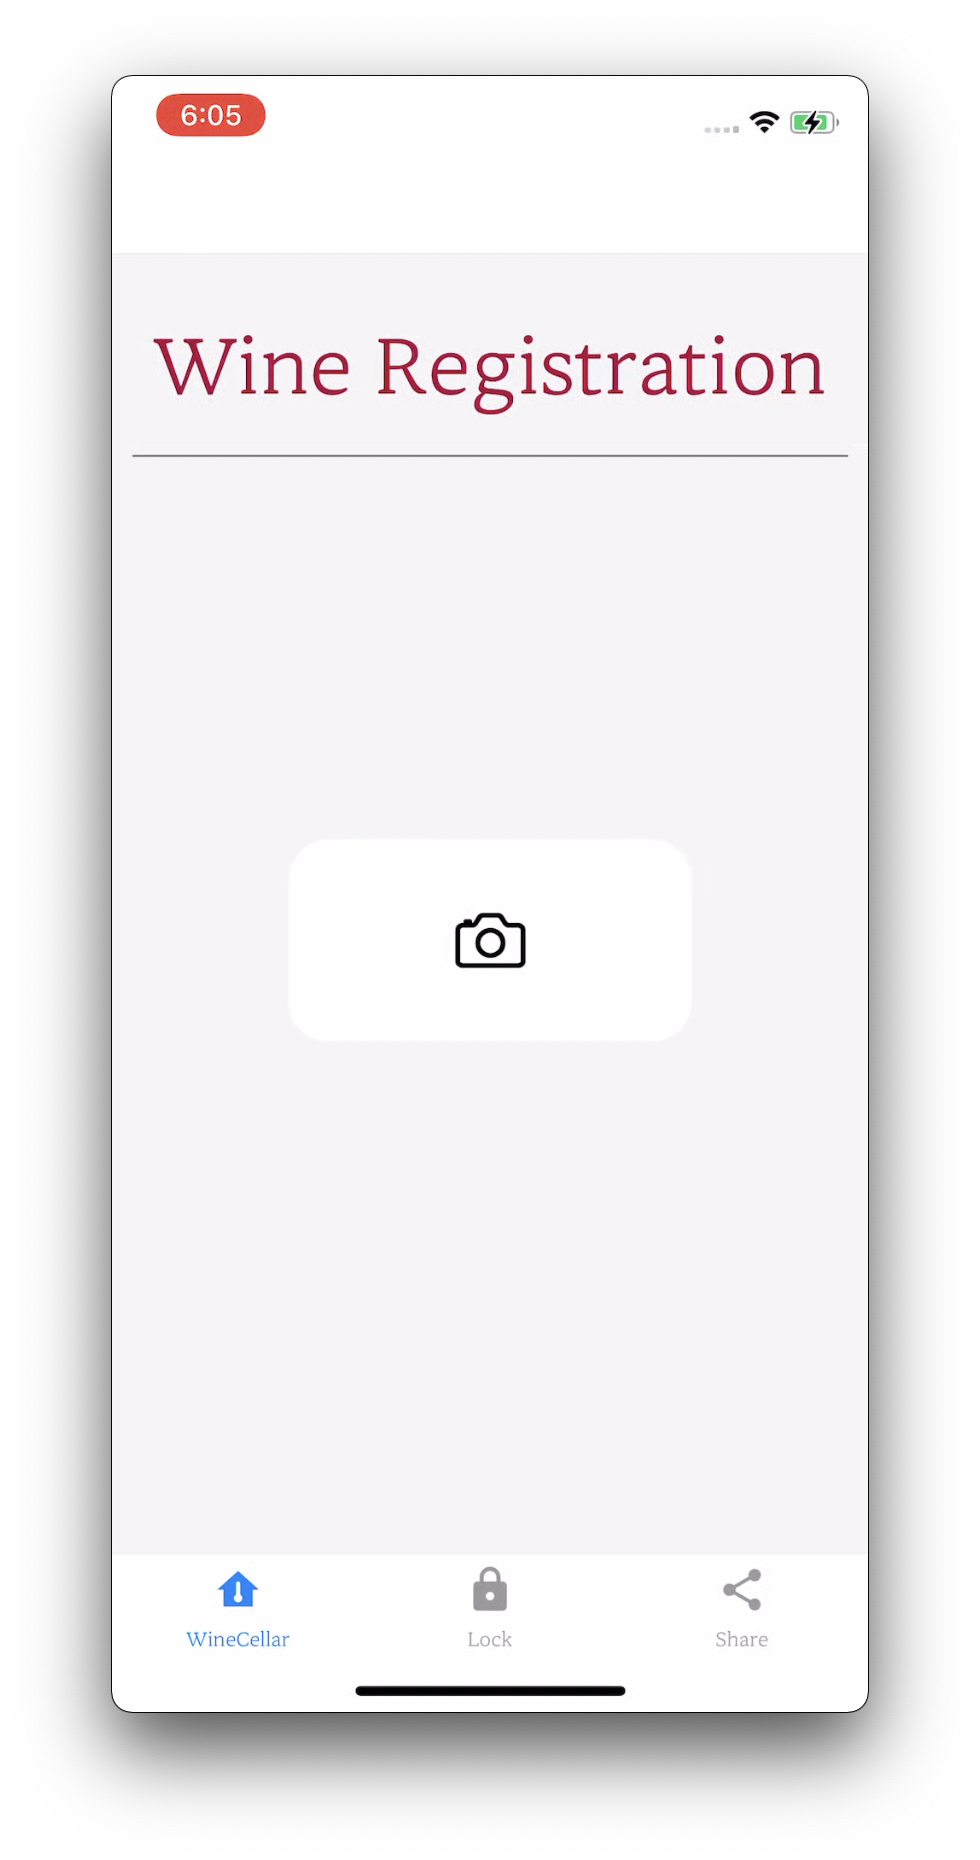
\includegraphics[width=5cm]{camera.png}}
        \centerline{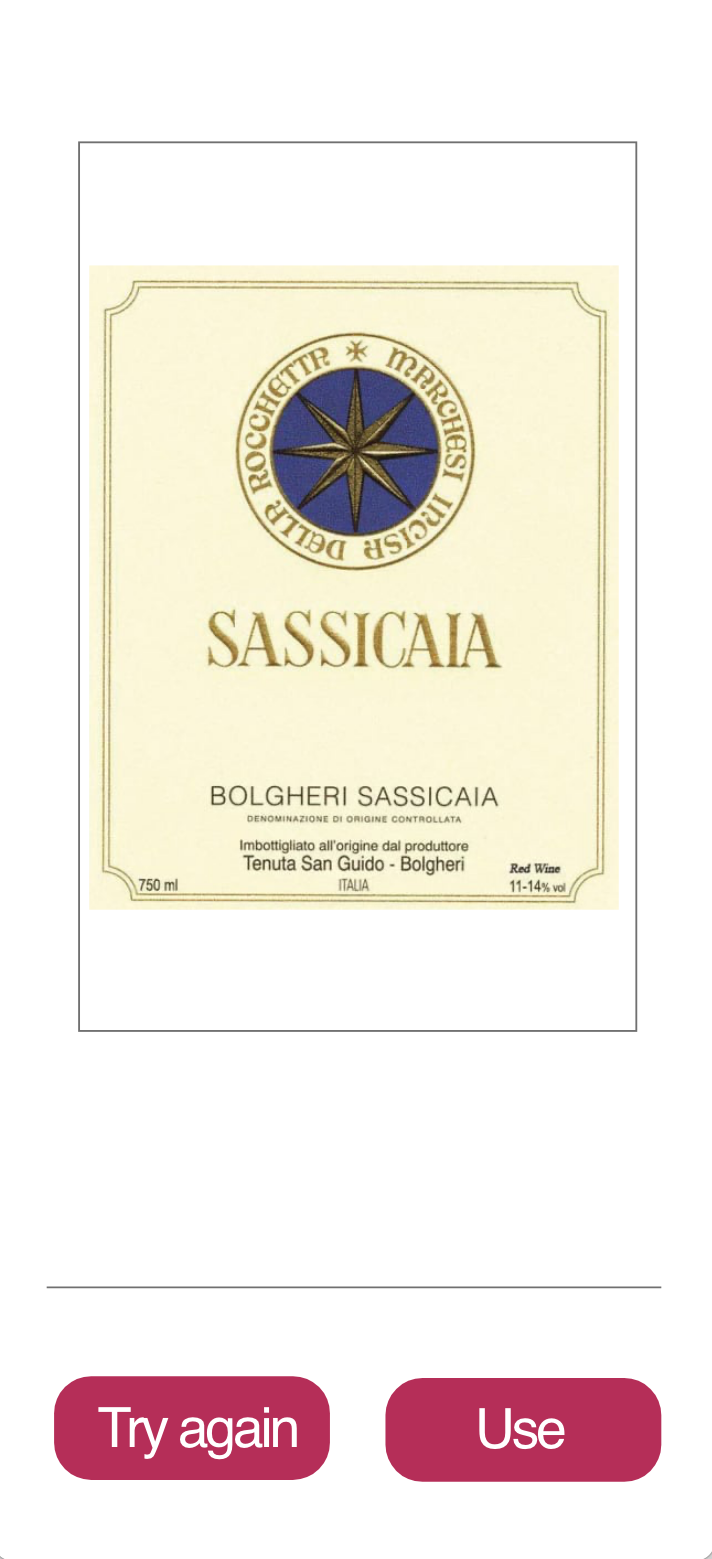
\includegraphics[width=5cm]{photo.png}}\begin{enumerate}
        \item User has to open camera application. After taking photo of wine label, user needs to determine whether to use the photo. If user presses ‘try again’ button, user goes to camera application again. Or else, user presses ‘use’ button, user starts wine registration step.
        \centerline{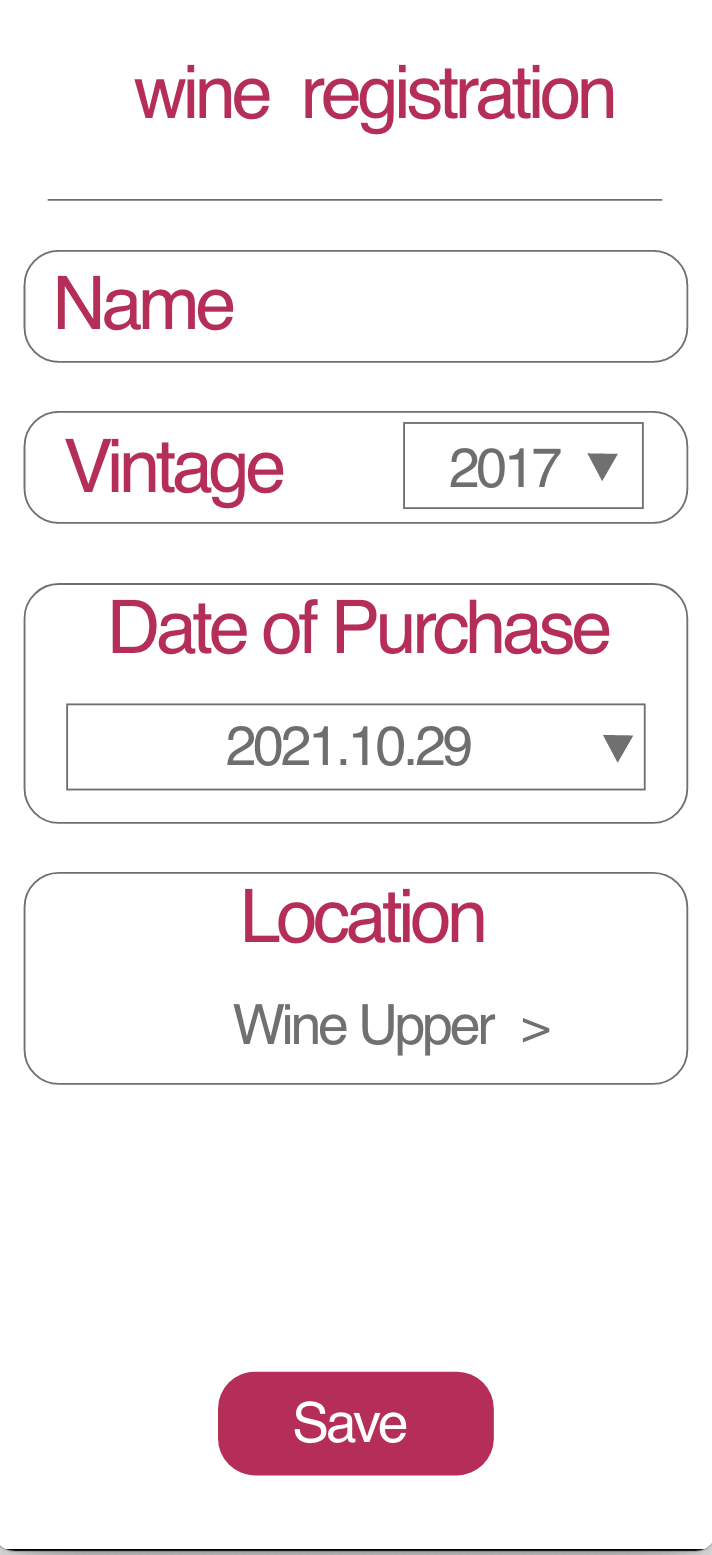
\includegraphics[width=5cm]{regiinfo.png}}
        \centerline{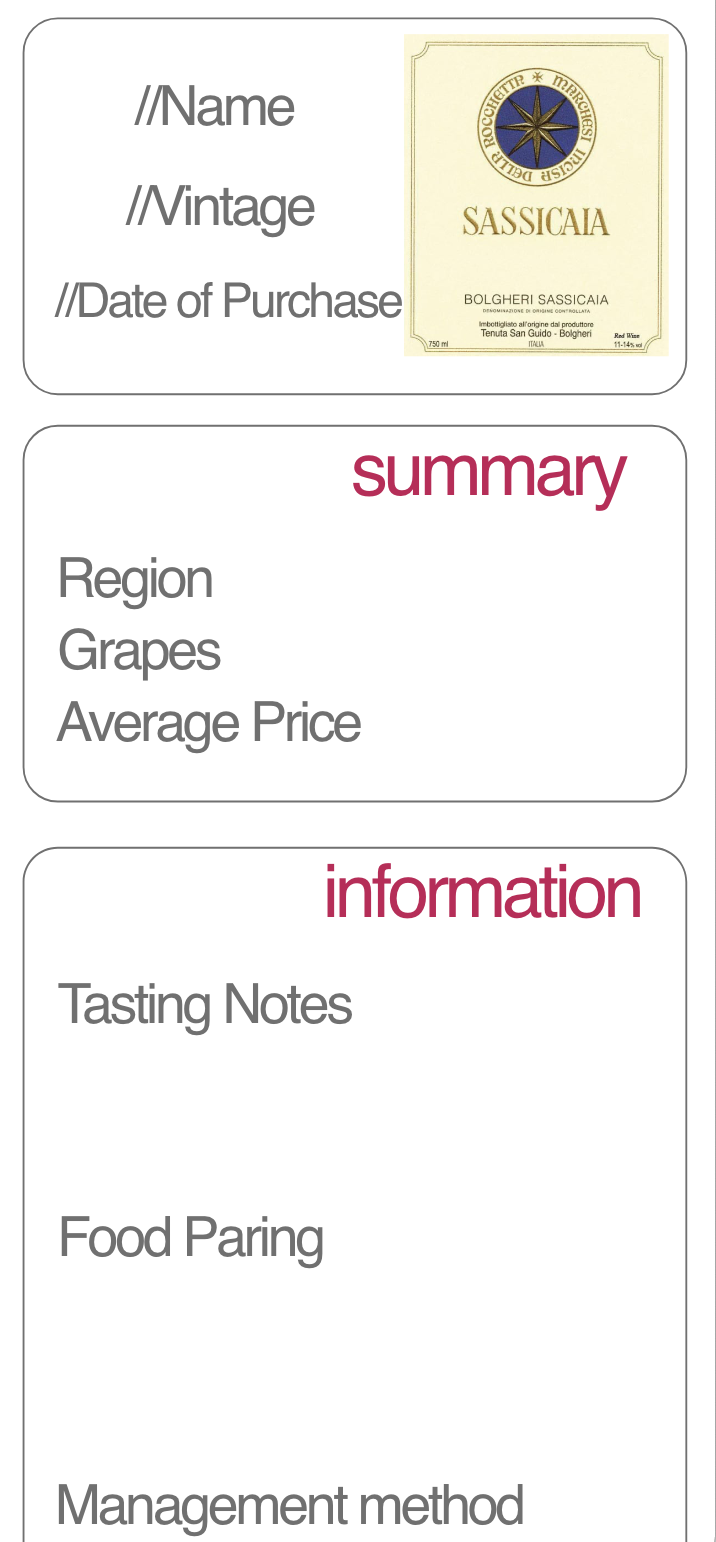
\includegraphics[width=5cm]{wineinfo.png}}
        \centerline{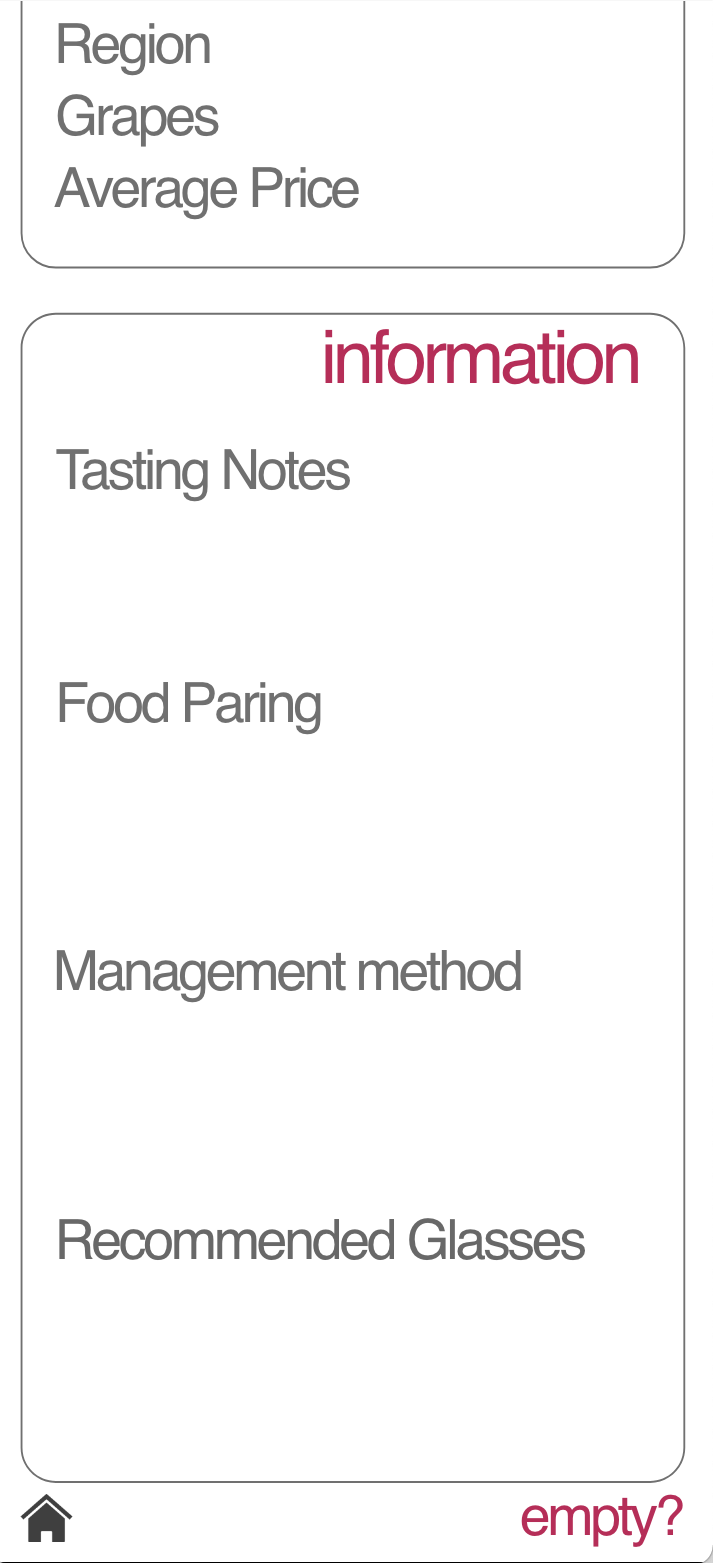
\includegraphics[width=5cm]{wineinfo2.png}}
        \item User starts wine registration step by step. Name of wine will be automatically completed by getting name from scanned-wine label database. But user needs to save vintage and date of purchase. Also, user needs to save location of wine, such as wine upper, wine lower. 
        \centerline{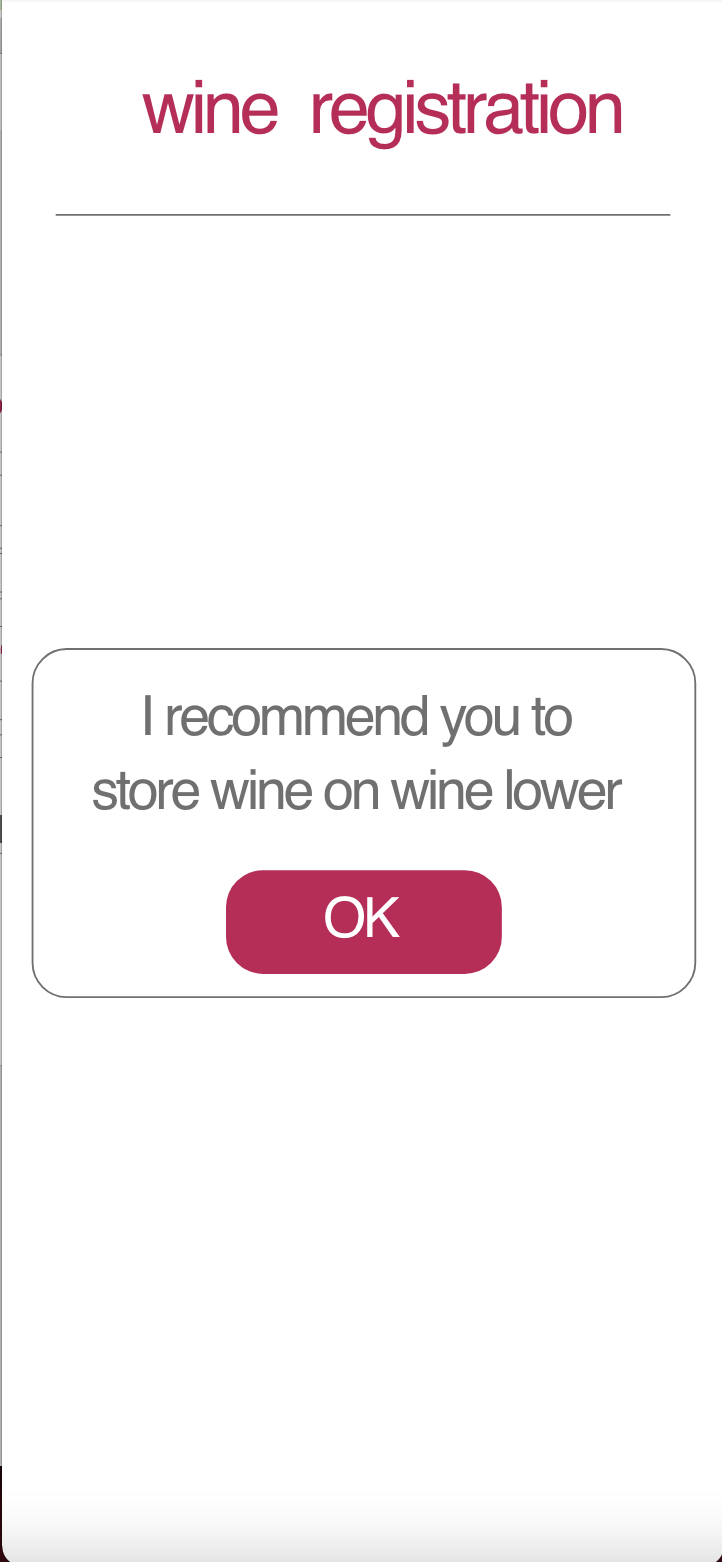
\includegraphics[width=5cm]{infocheck.png}}
        \item When user saves these information, pop up window may appear to user. If user saves wine in appropriate floor.
        \end{enumerate}
        
        \item \textit{\textbf{Wine cellar Lock} (Lock icon)}\\
        \centerline{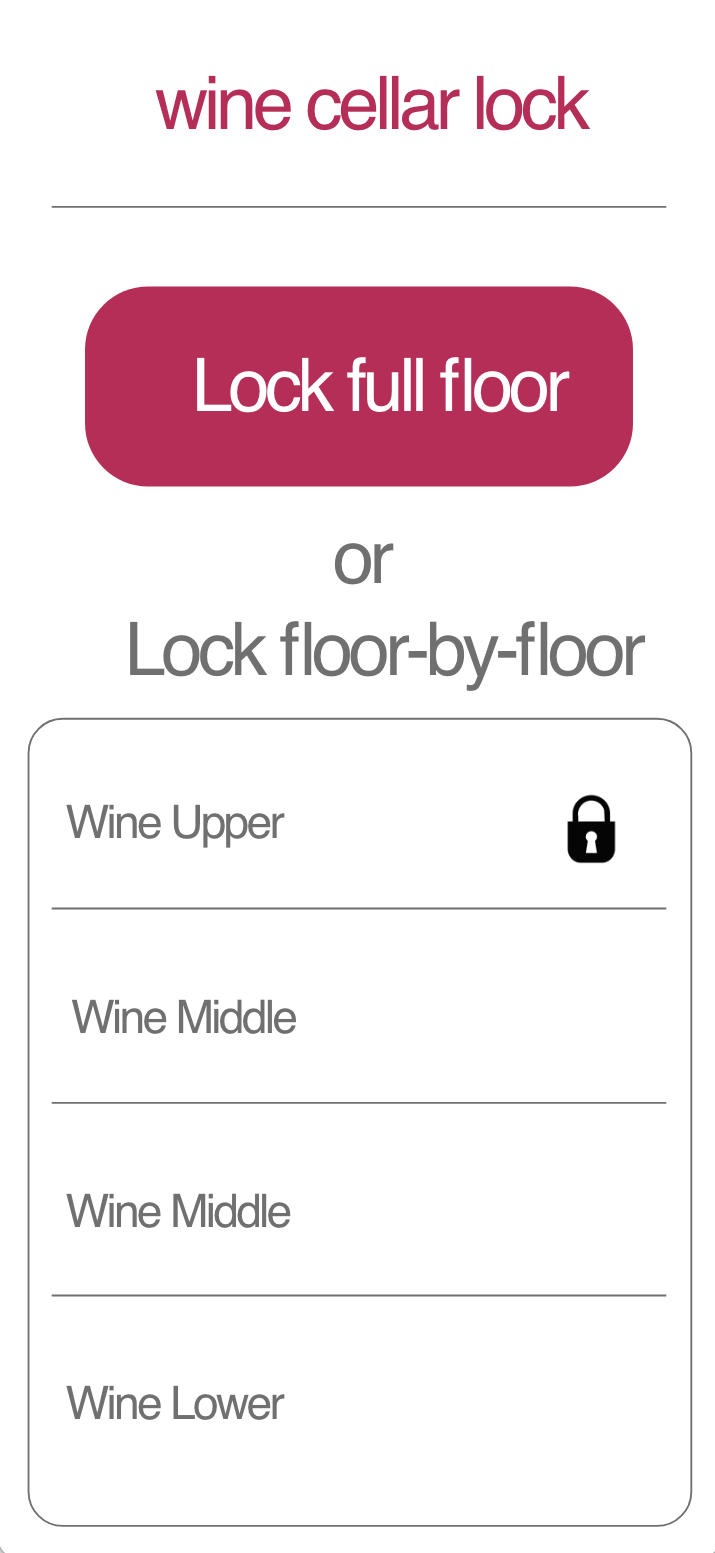
\includegraphics[width=5cm]{lock.png}}
        When user clicks lock icon, user goes to ‘wine cellar lock’. If user wants to lock full floor, user can click ‘lock full floor button’. Or else, user can lock floor by floor by clicking each lock button.
        \item \textit{\textbf{Wine Recommendation} (Alarm icon)}\\
        \centerline{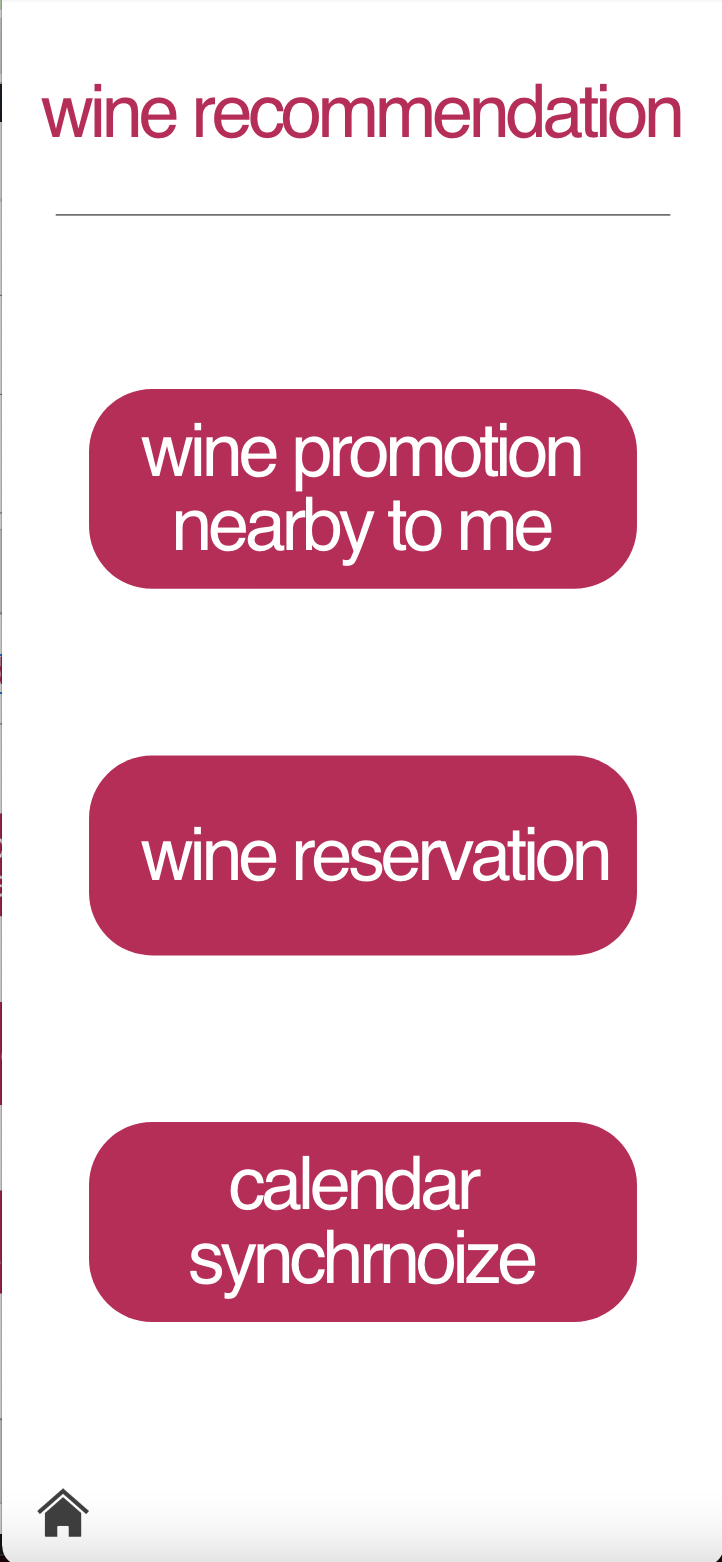
\includegraphics[width=5cm]{winerec.png}}
        On the wine recommendation page, users can go to pages that check nearby wine-related events (e.g., discounts), get information about 'nearby wine shops', 'buy wine or make reservations', and 'recommend wine which fits in with their schedules'. \begin{enumerate}
            \item \textit{Wine promotion nearby to me}
            \begin{enumerate}
            \centerline{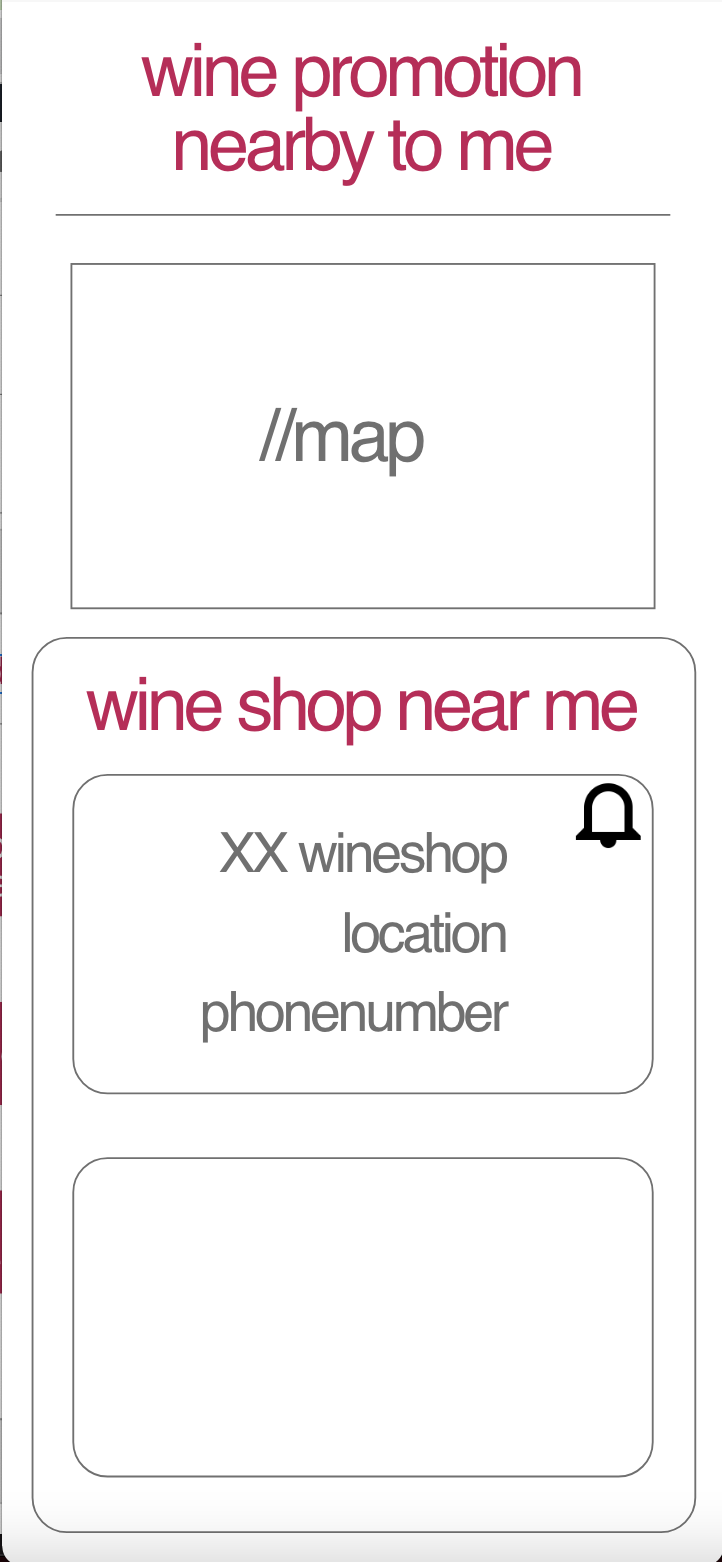
\includegraphics[width=5cm]{winepromo.png}}
                \item The application requests the user's location information. If the user allows the request, the map displays wine promotion around the user. 
                \item The 'wine shop nearby to me' view under the 'map' view displays wine shops around the user. Users can set alarms for each wine shop by clicking the bell icon on the top right. If an event or promotion is held at a wine shop with an alarm set, the application sends a notification to the user. 
                \centerline{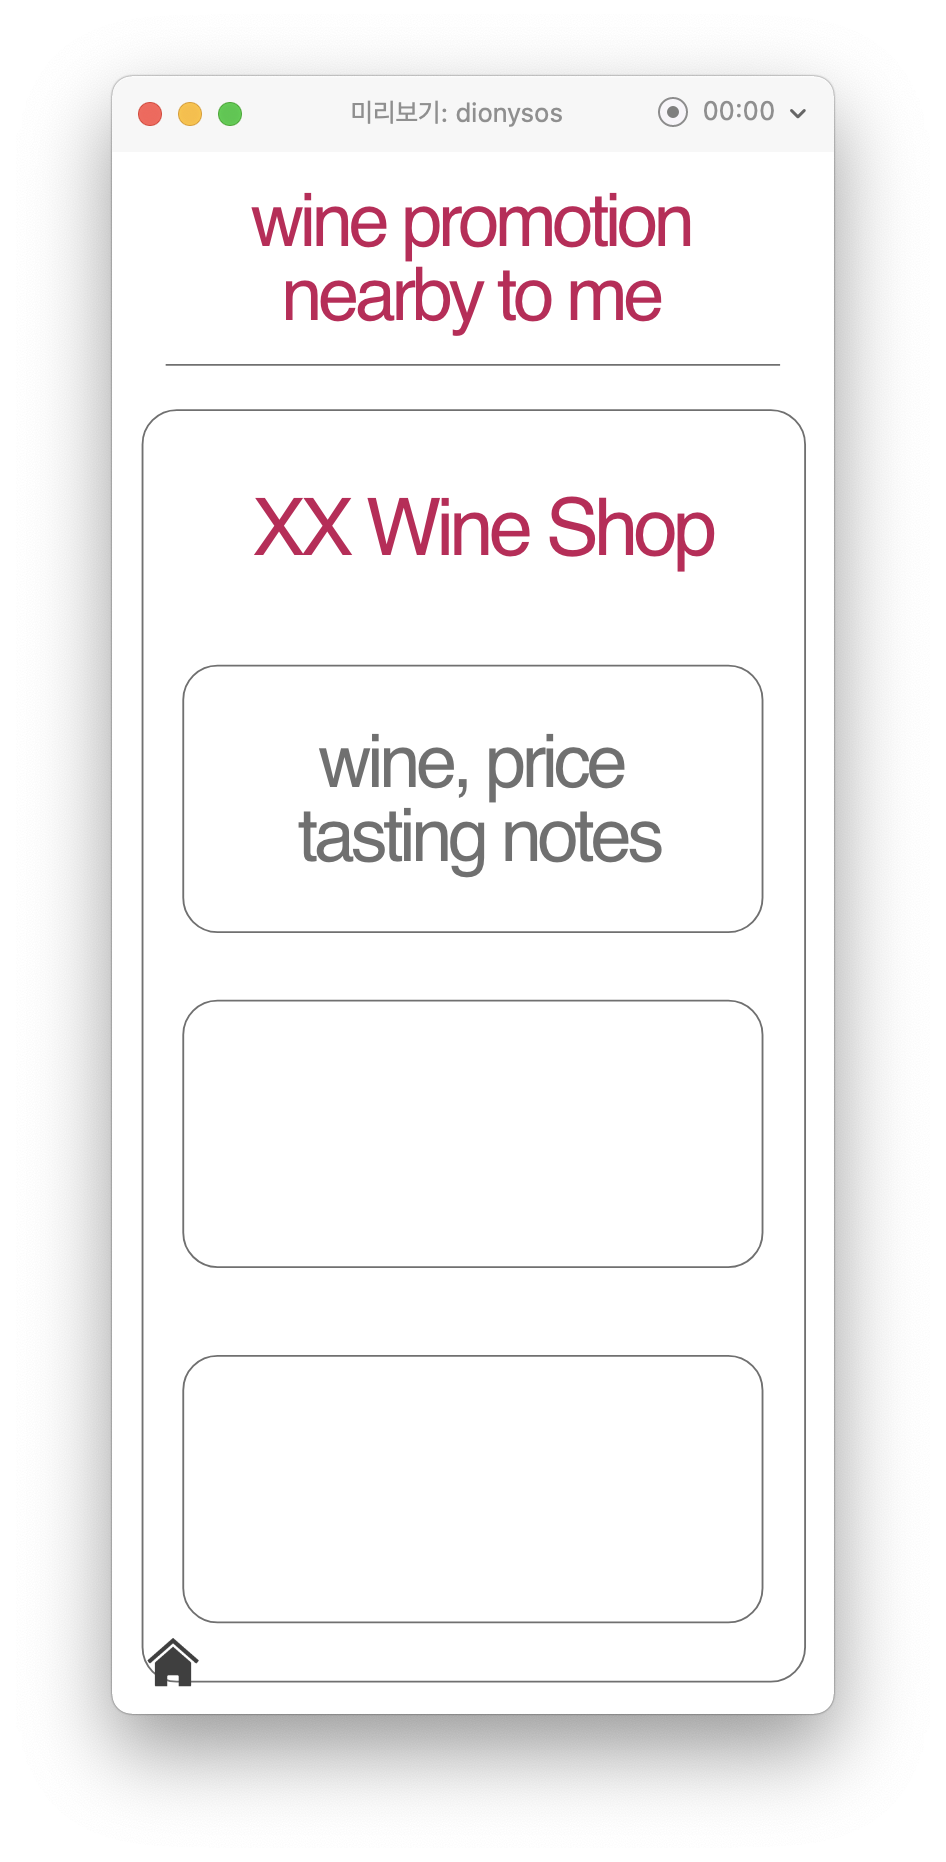
\includegraphics[width=5cm]{winepromoalarm.png}}
                \item When the user clicks the notification, wines corresponding to the event at the wine shop are displayed. The app shows the name, price, and testing notes of the wine.
            \end{enumerate}
            
            \item \textit{Wine reservation}\\
            On the Wine Reservation page, users can search for and reserve the wine they want to purchase. 
            \begin{enumerate}
            \centerline{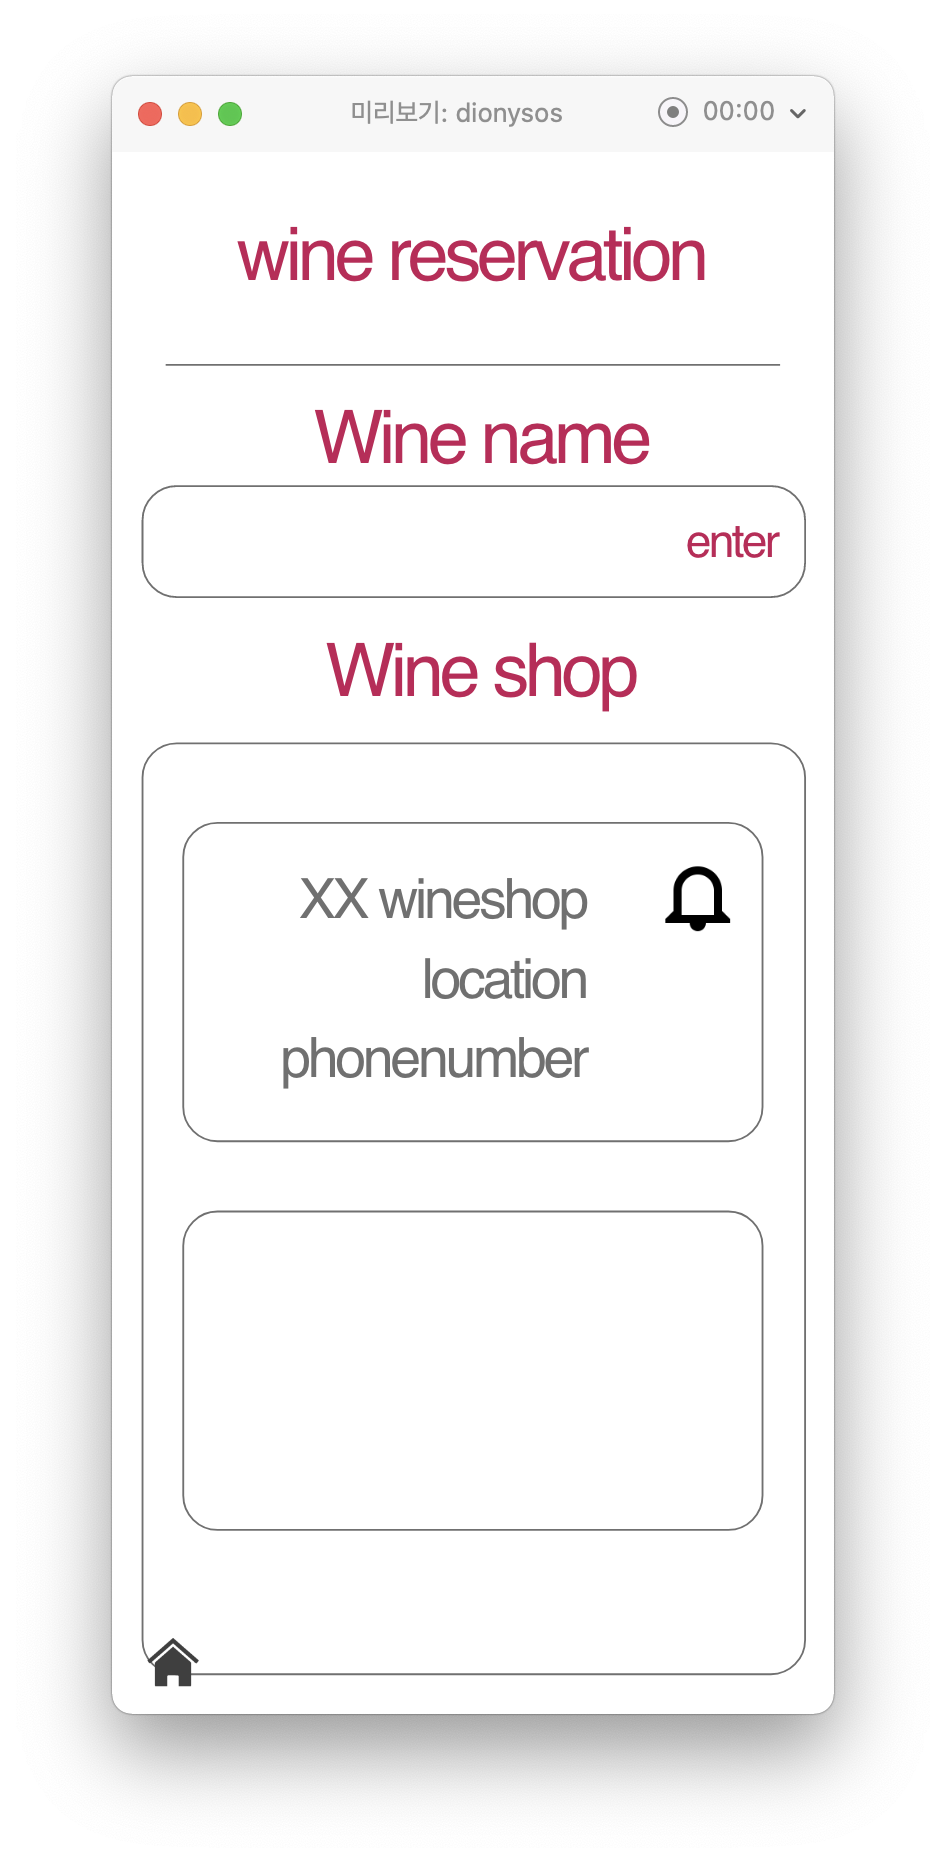
\includegraphics[width=5cm]{wineres.png}}
                \item The user can search for wine by entering the name of the wine. When the user writes the name of the wine and presses the enter button, the app shows several shops where wine entered by the user can be purchased.\\
                
                The user can press the bell button on the upper right in each wine shop view to receive a notification whenever the wine he or she wants becomes available for purchase. App sends notification if the wine user wants has arrived at the wine shop.
                \item Alarm\\
                \centerline{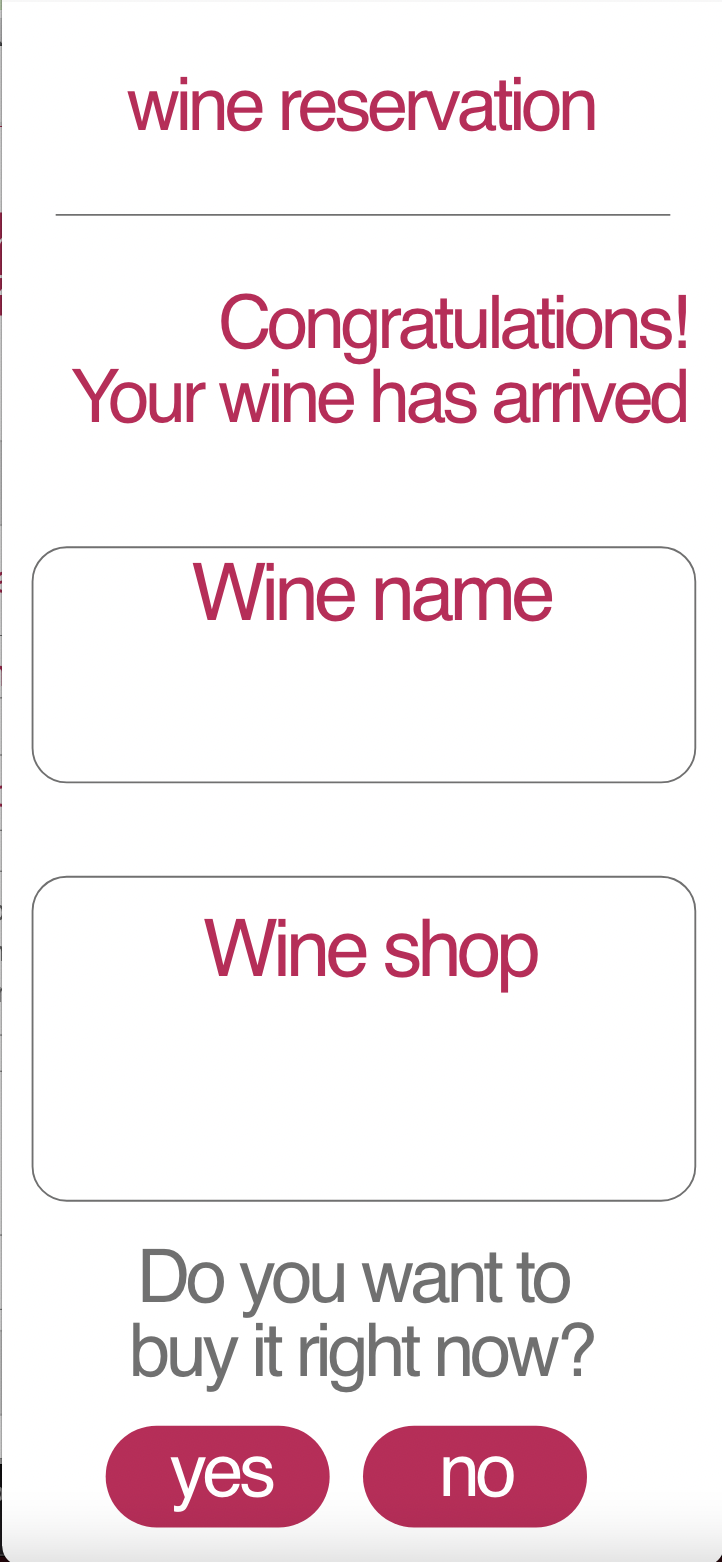
\includegraphics[width=5cm]{winearrive.png}}
                When wine that user wants arrives at the wine shop where the user presses the bell button and becomes available, the app sends a notification to the user. When the user clicks the notification, it goes to the Congratulation page. On the Congratulation page, users can see the name of the wine and the store they reserved, and the question of whether to purchase it 'right now'.
                \item Reservation\\
                \centerline{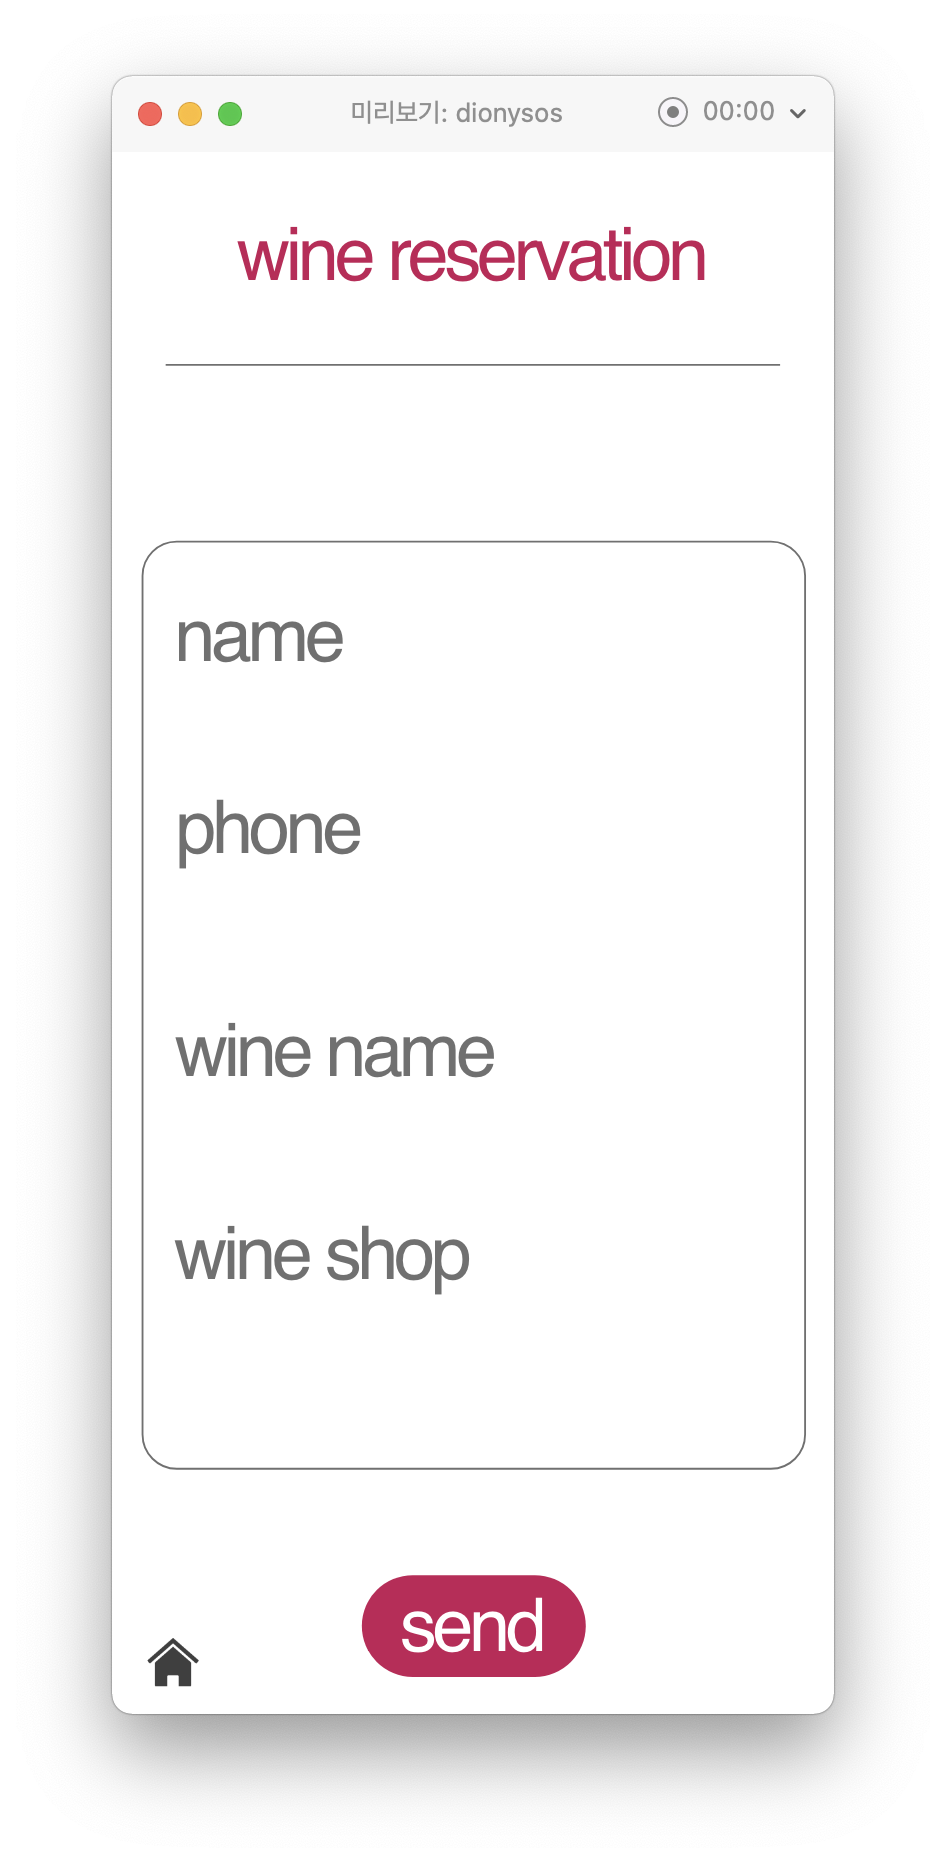
\includegraphics[width=5cm]{winebuy.png}}
                If the user presses yes to show his intention to purchase it right now, go to the 'wine reservation' page. On the 'wine reservation' page, the user writes down his name, phone number, name of wine to purchase, and name of the store to purchase wine and presses the send button. The information pressed here is sent to the corresponding wine store. 
            \end{enumerate}
            \item \textit{Calendar synchronize}\\
            \centerline{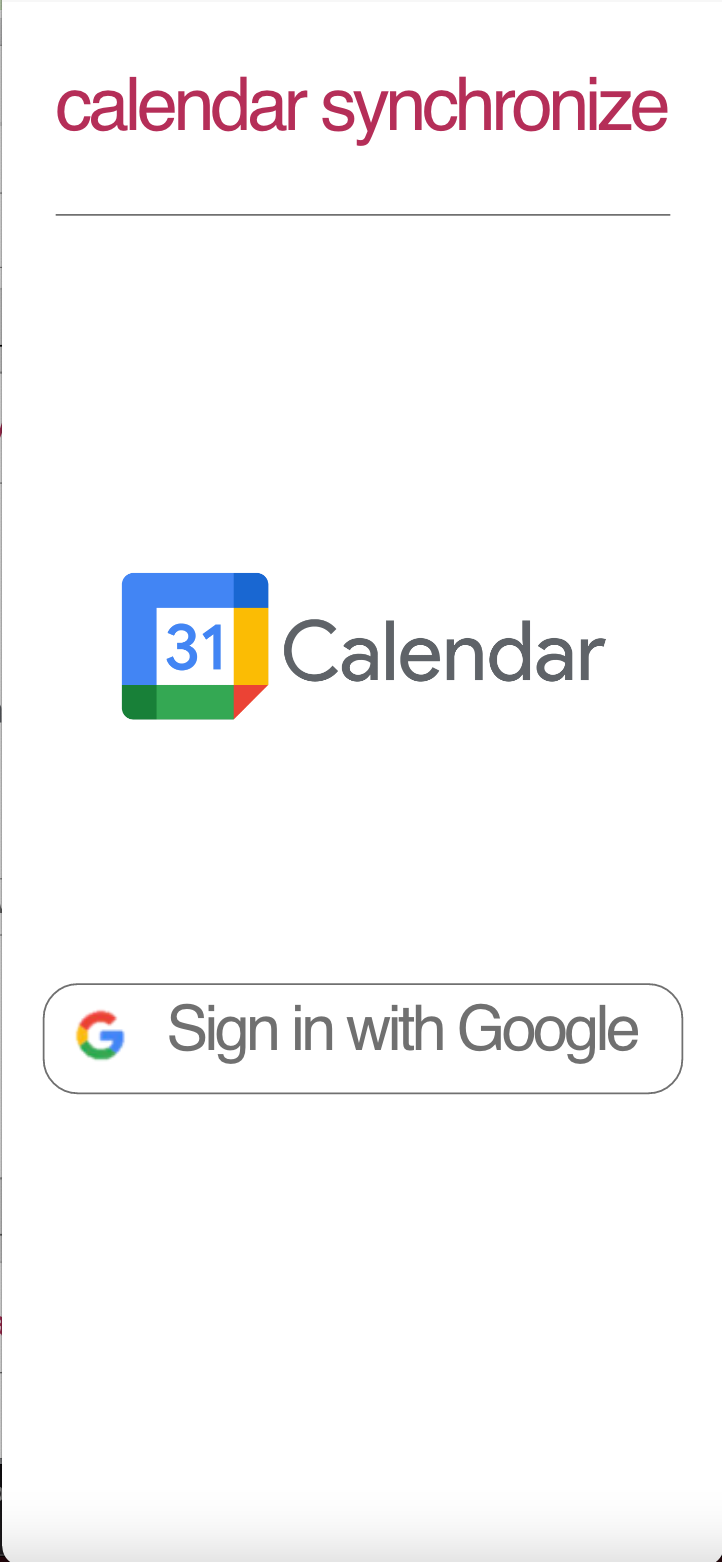
\includegraphics[width=5cm]{calendar.png}}
            By logging in with their Google account, users can link this app with their Google Calendar. 
\centerline{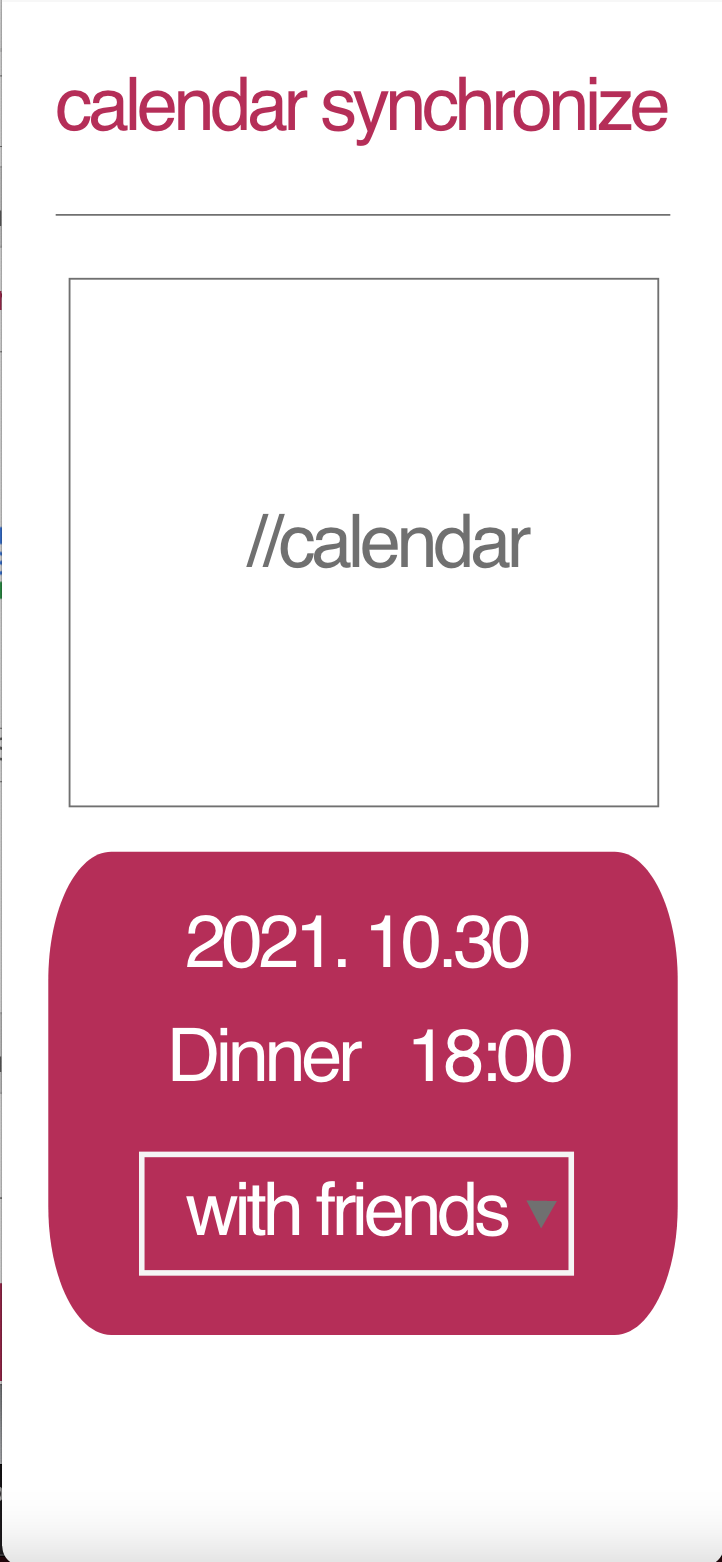
\includegraphics[width=5cm]{calendar2.png}}
Using Google-Calendar-api, the application displays the calendar of current month. When the user clicks on the day with schedule, the schedule of the day is displayed in the view under the calendar. The daily schedule indicates the date and time, the purpose of the schedule (e.g., evening, party), and who users are meeting with.
\centerline{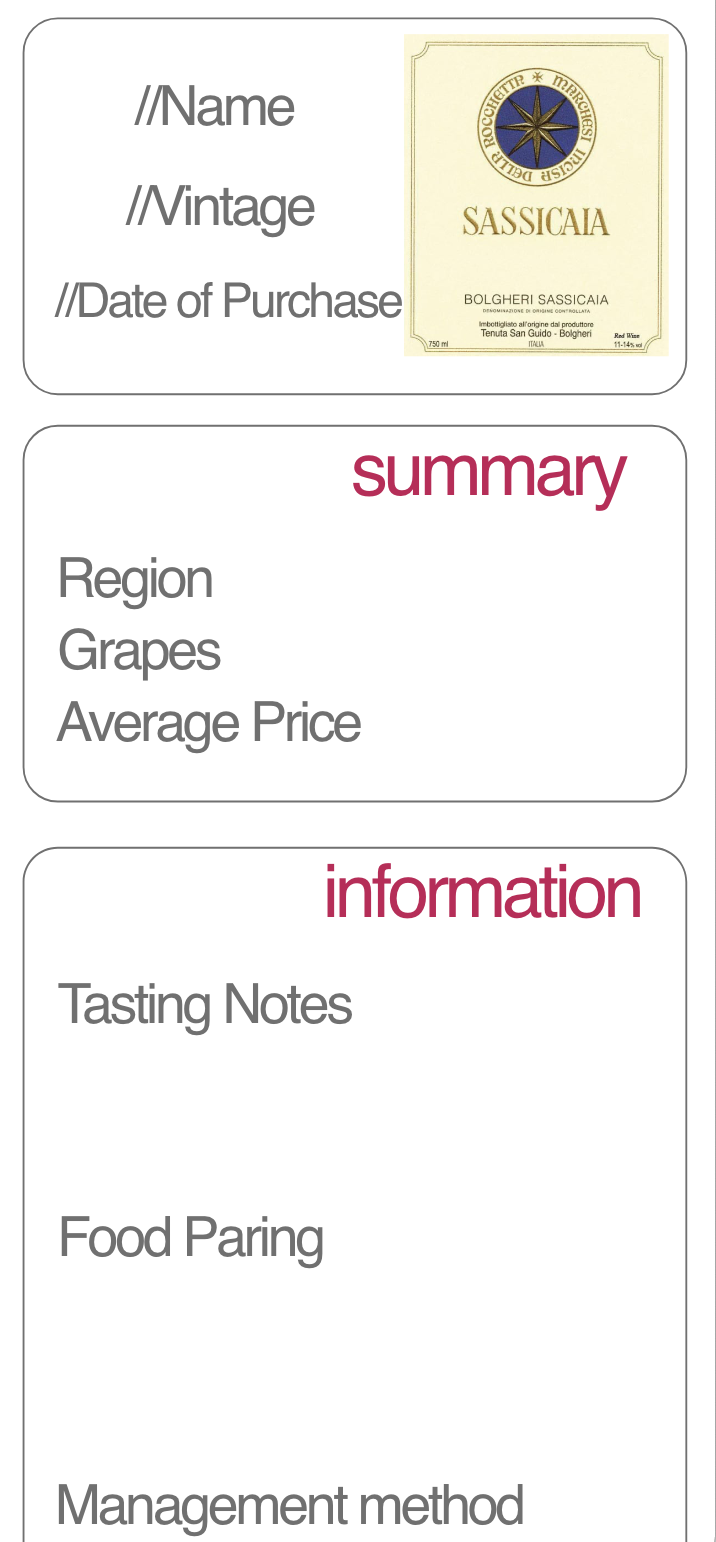
\includegraphics[width=5cm]{wineinfo.png}}
The app focuses on 'people' who are together that day. The recommended wine depends on who the users are with that day. People who share schedule with users are highlighted with white lines. If the user presses the highlighted part (button), the app goes to the 'wine information' page of the recommended wine.
        \end{enumerate}
        \item \textit{\textbf{Share} (Share icon)}\\
        \centerline{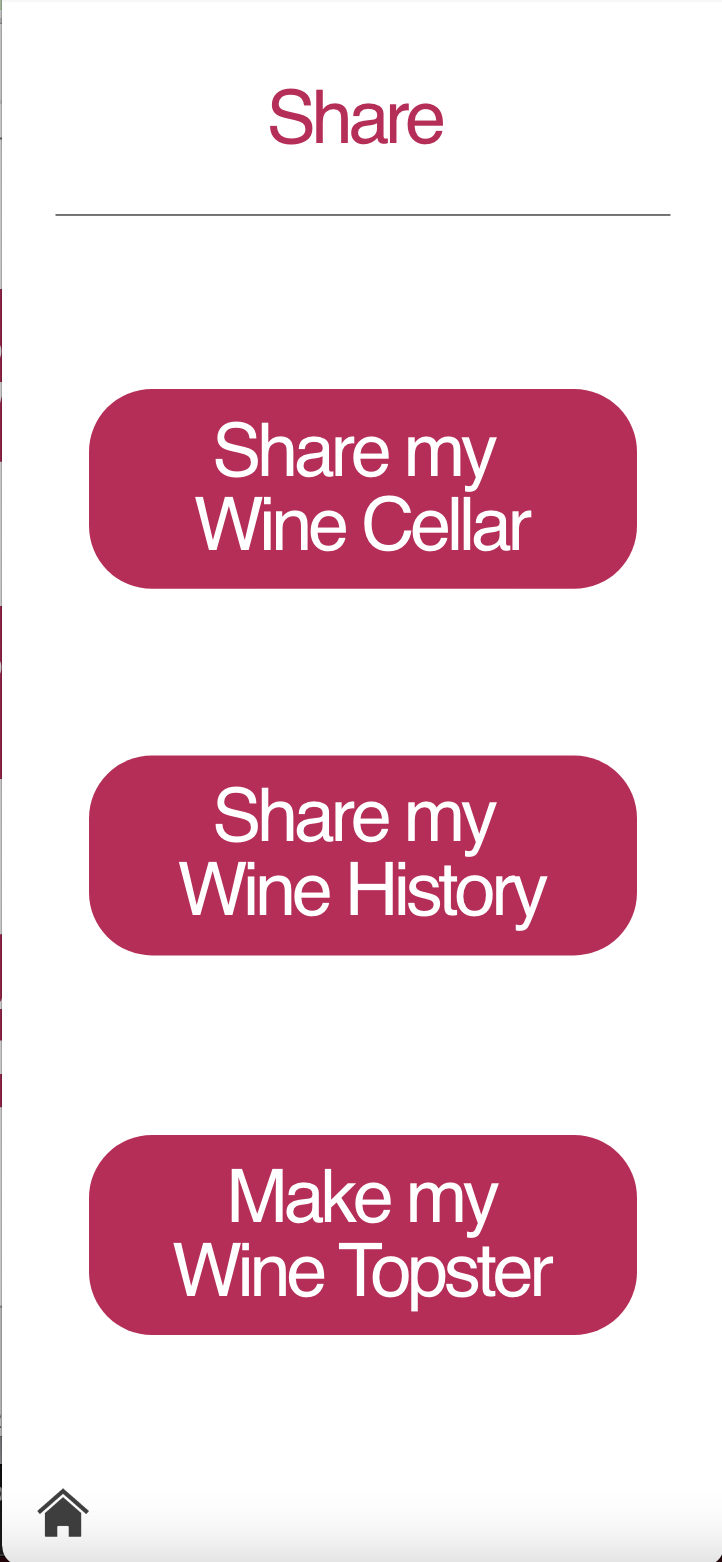
\includegraphics[width=5cm]{share.png}}
        Share, which is consisted of ‘share my Wine cellar’, ‘share my Wine history’, and ‘make my Wine Topster’, lets user to share wine-related images in Instagram, Facebook, Twitter and saves images to gallery in common. When user shares these images, hashtag \#LGwinecellar, \#MyWineCellar, and \#DIOnyoS will be automatically completed. And it can lead to promotion of wine cellar and application DIOnyoS.
        \begin{enumerate}
        \item \textit{Share my Wine Cellar}\\
        \centerline{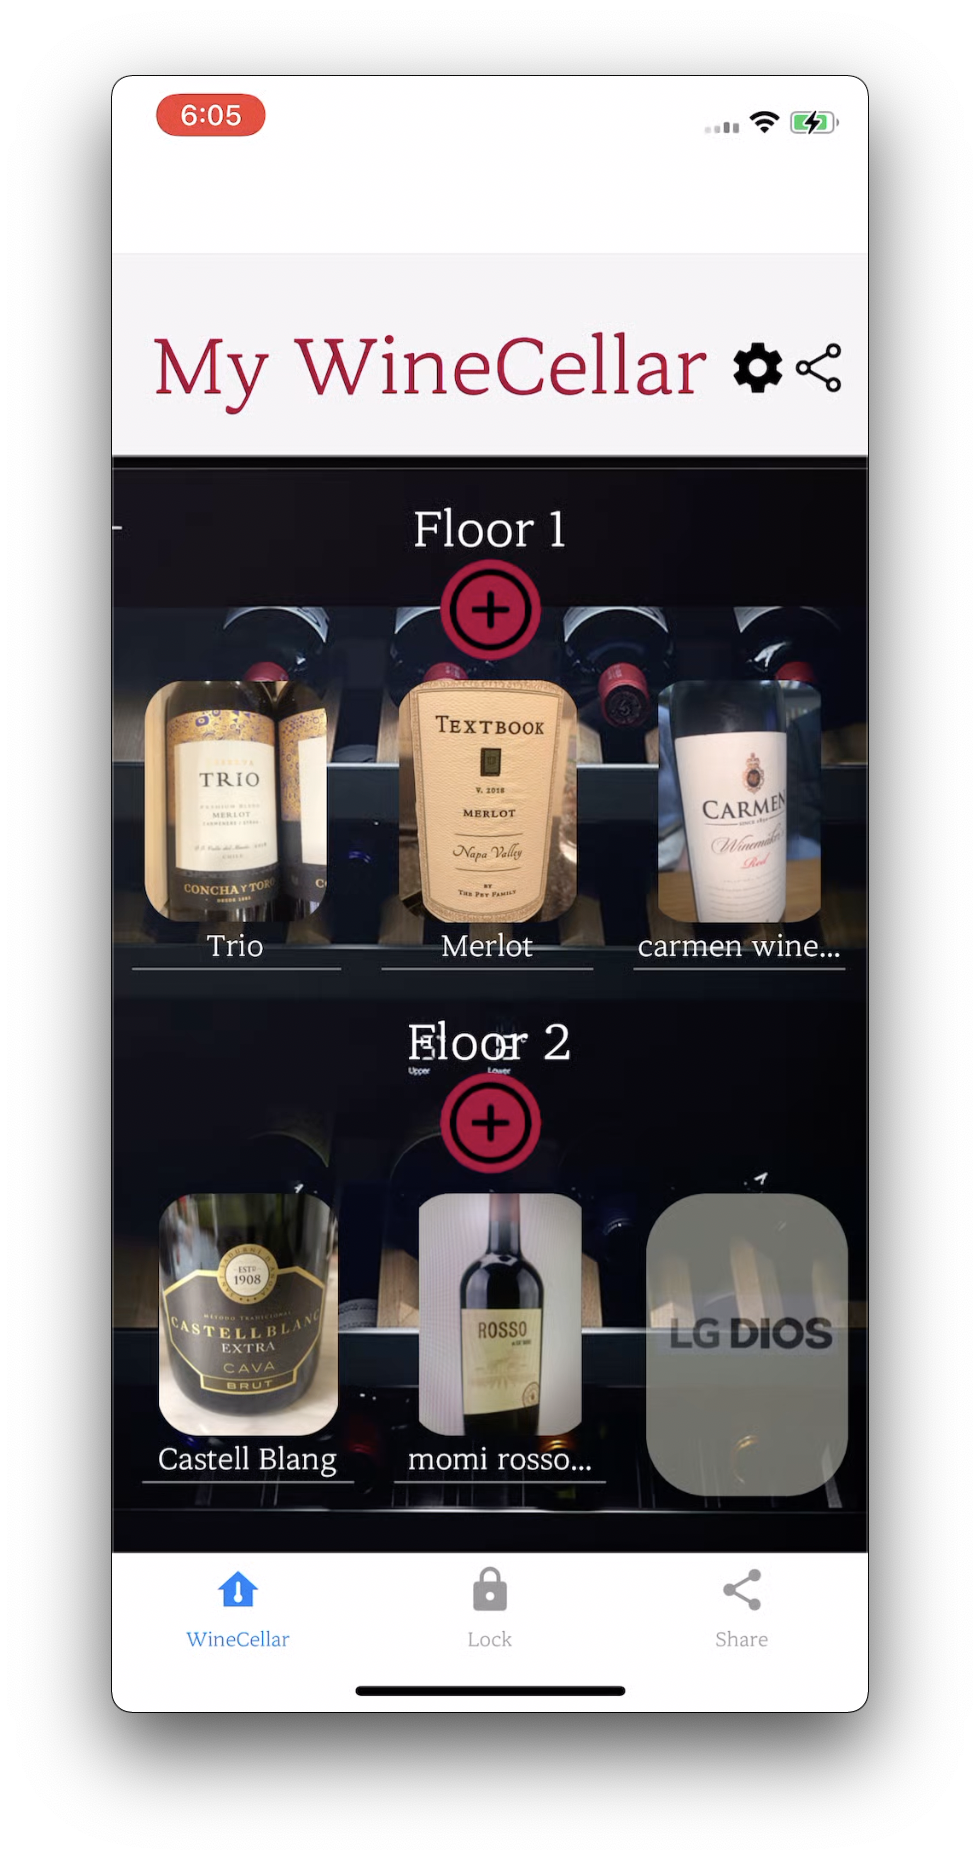
\includegraphics[width=5cm]{sharecel.png}}
        Share my Wine Cellar lets user to take screentshot of ‘My WineCellar’, which is main page.
        \item \textit{Share my Wine History}\\
        \begin{enumerate}
            \item Cork\\
            \centerline{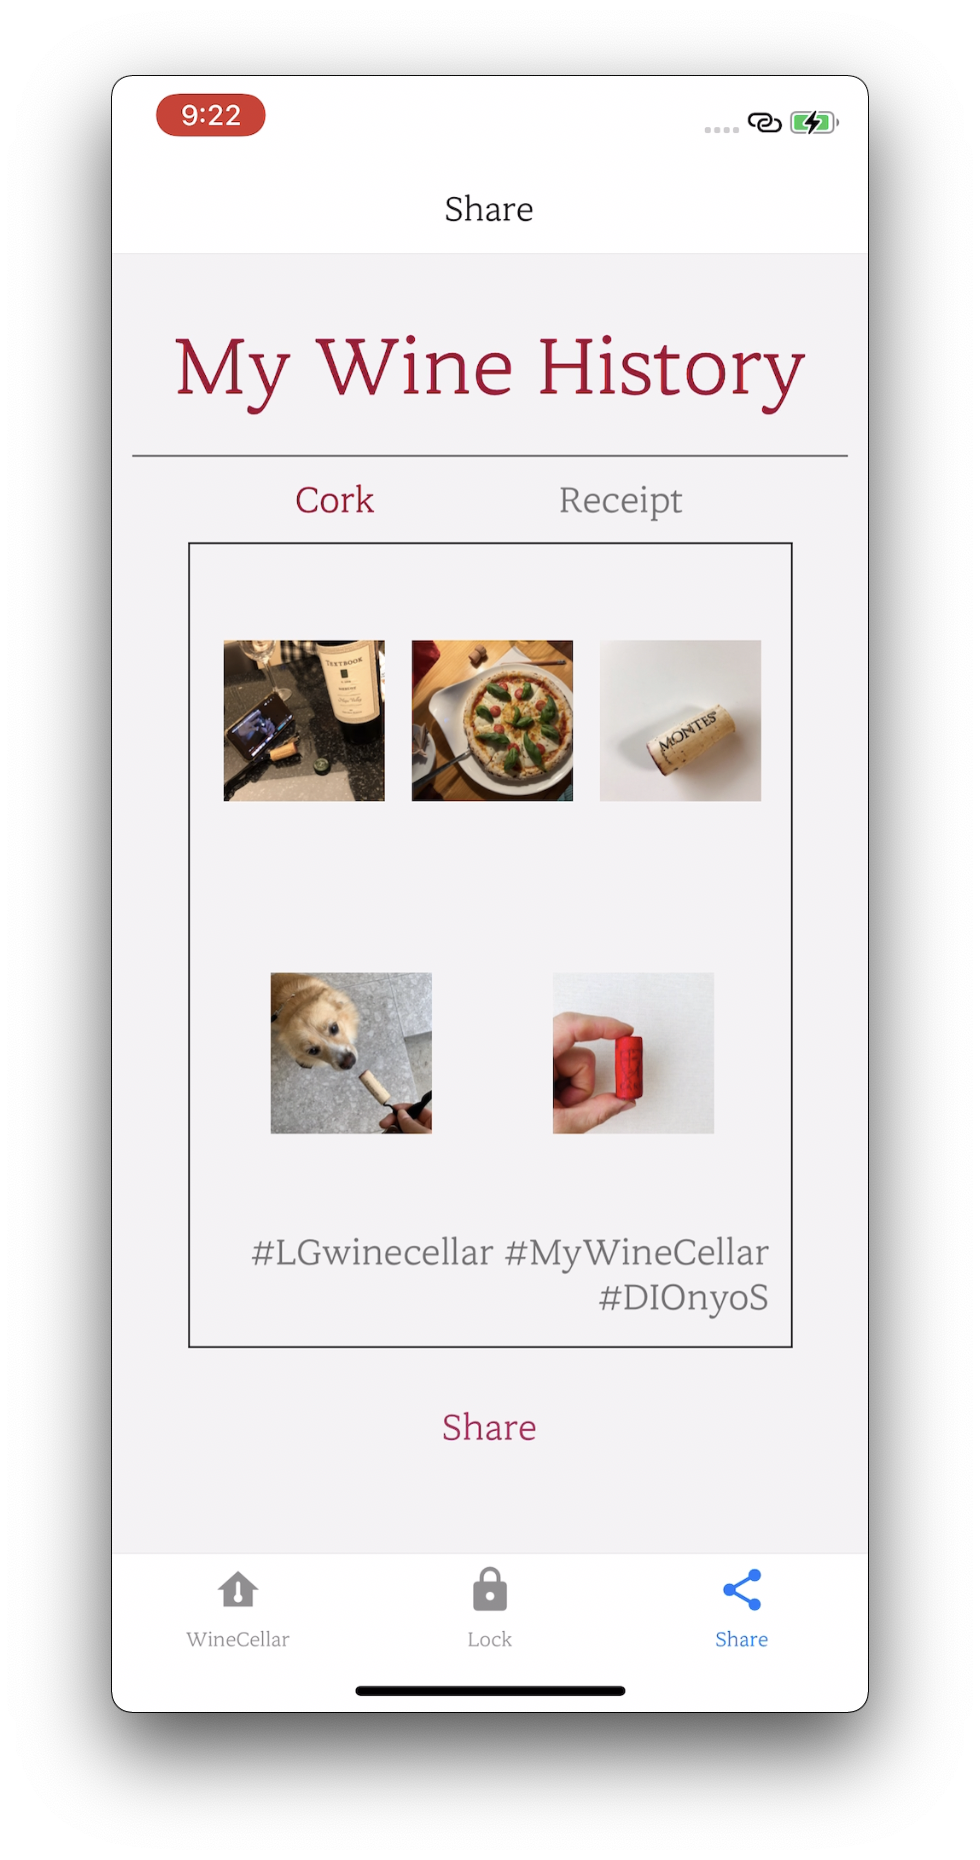
\includegraphics[width=5cm]{sharecork.png}}
            The number of wine which user has drunk until now appears as the images of cork. And it will look like loyalty card. So, the more user drink, the more cork user can collect.
            \item Receipt\\
            \centerline{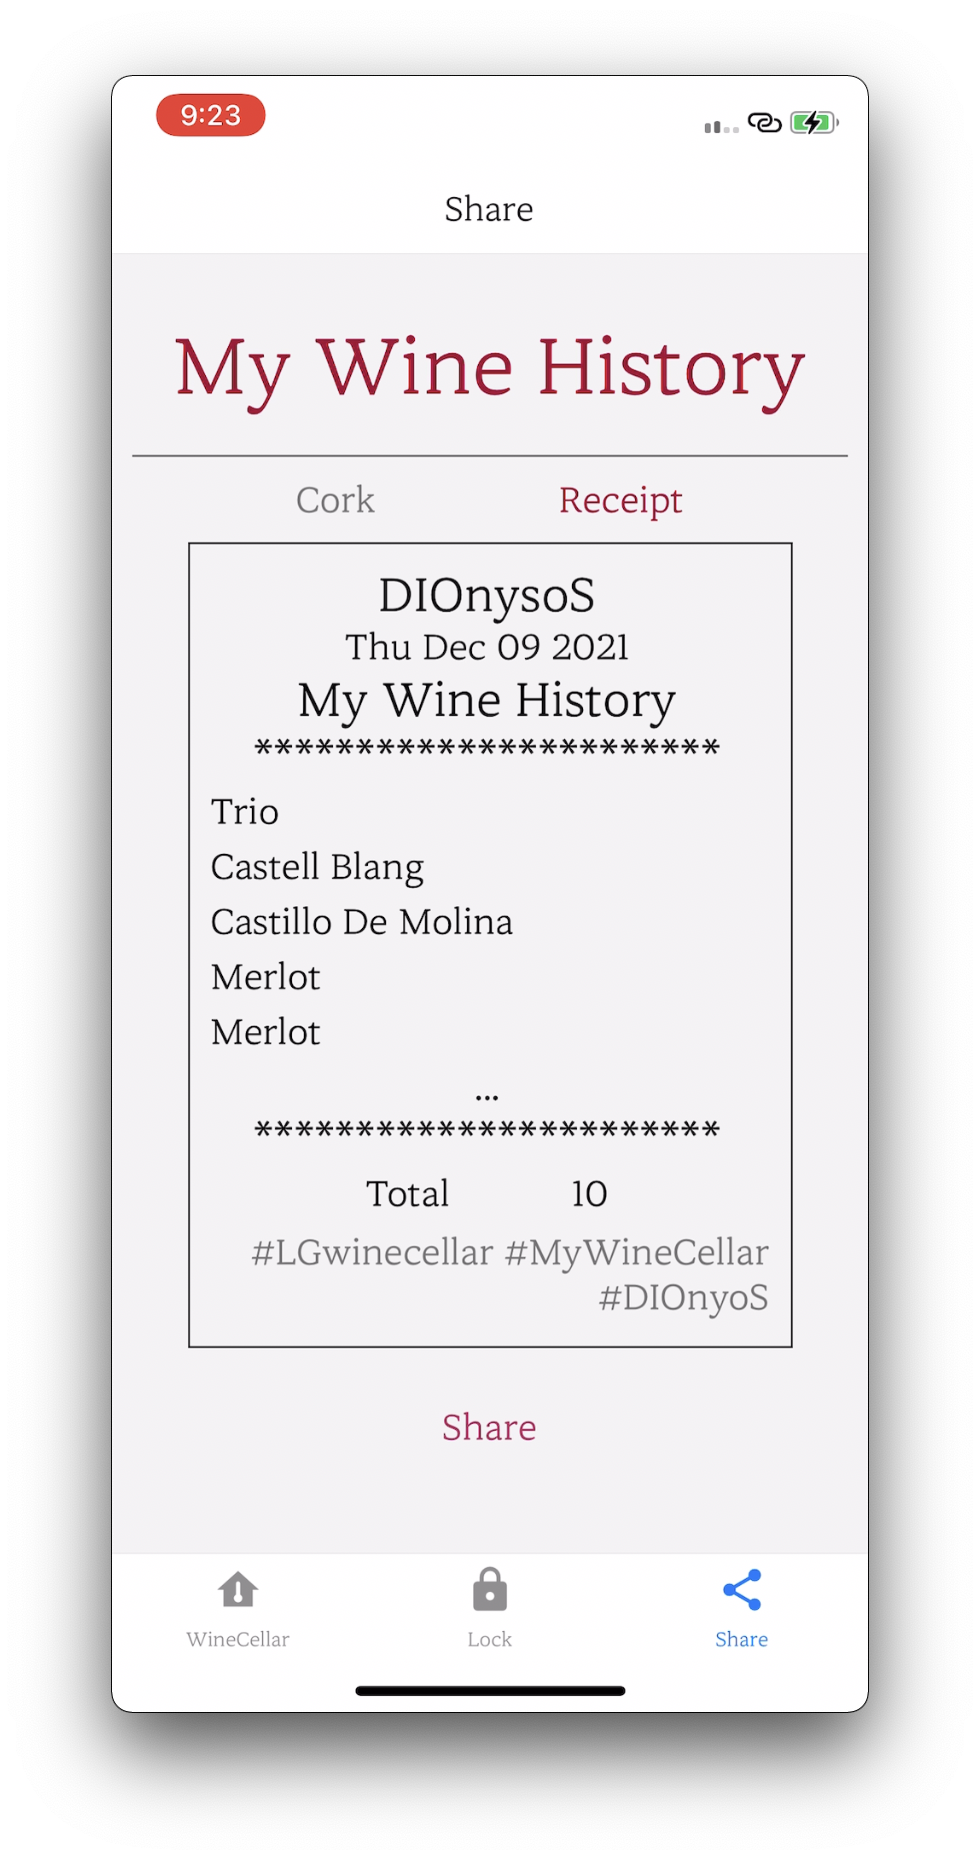
\includegraphics[width=5cm]{sharerec.png}}
            Wine which user has drunk until now appears as the format of receipt. Receipt is consisted of name, number and price of each wine. And total amount and price of wine will appear at the bottom of receipt.
        \end{enumerate}
        \item \textit{Make my Wine Topster}
        \begin{enumerate}
        \centerline{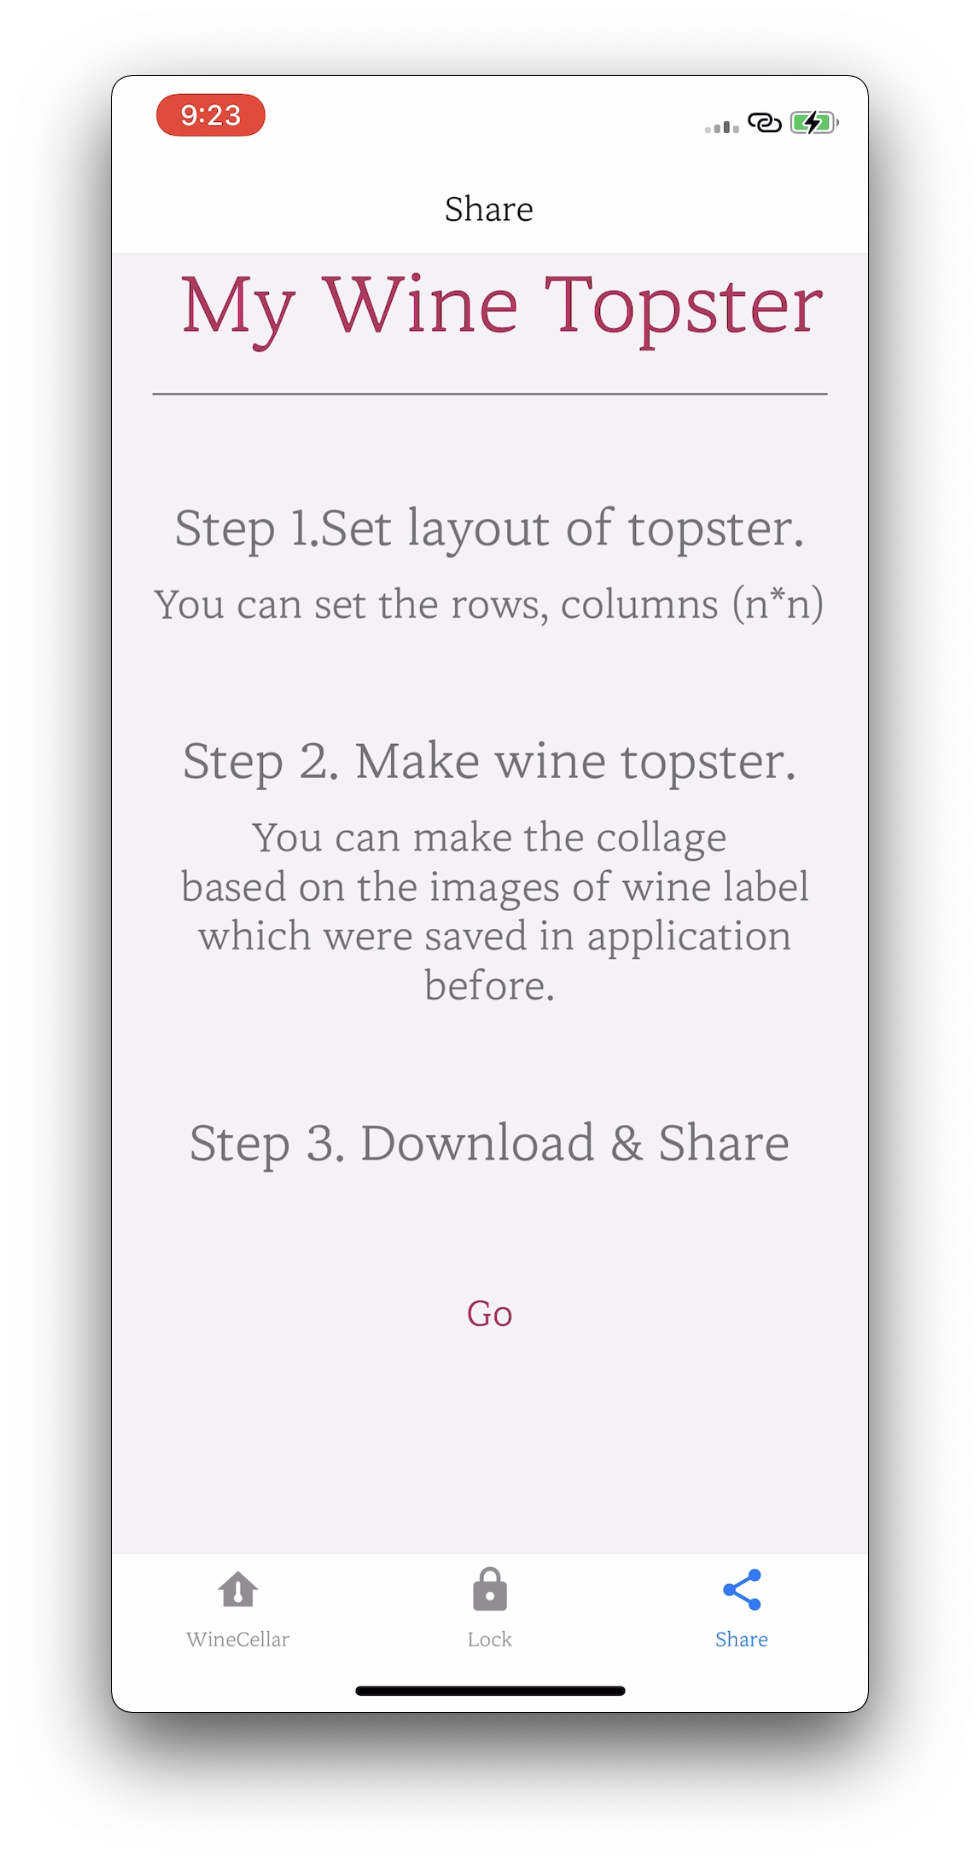
\includegraphics[width=5cm]{sharetop.png}}
      
            \item Description of making topster will appear. When user clicks ‘Go’ button, user can start making his own topster.
              \centerline{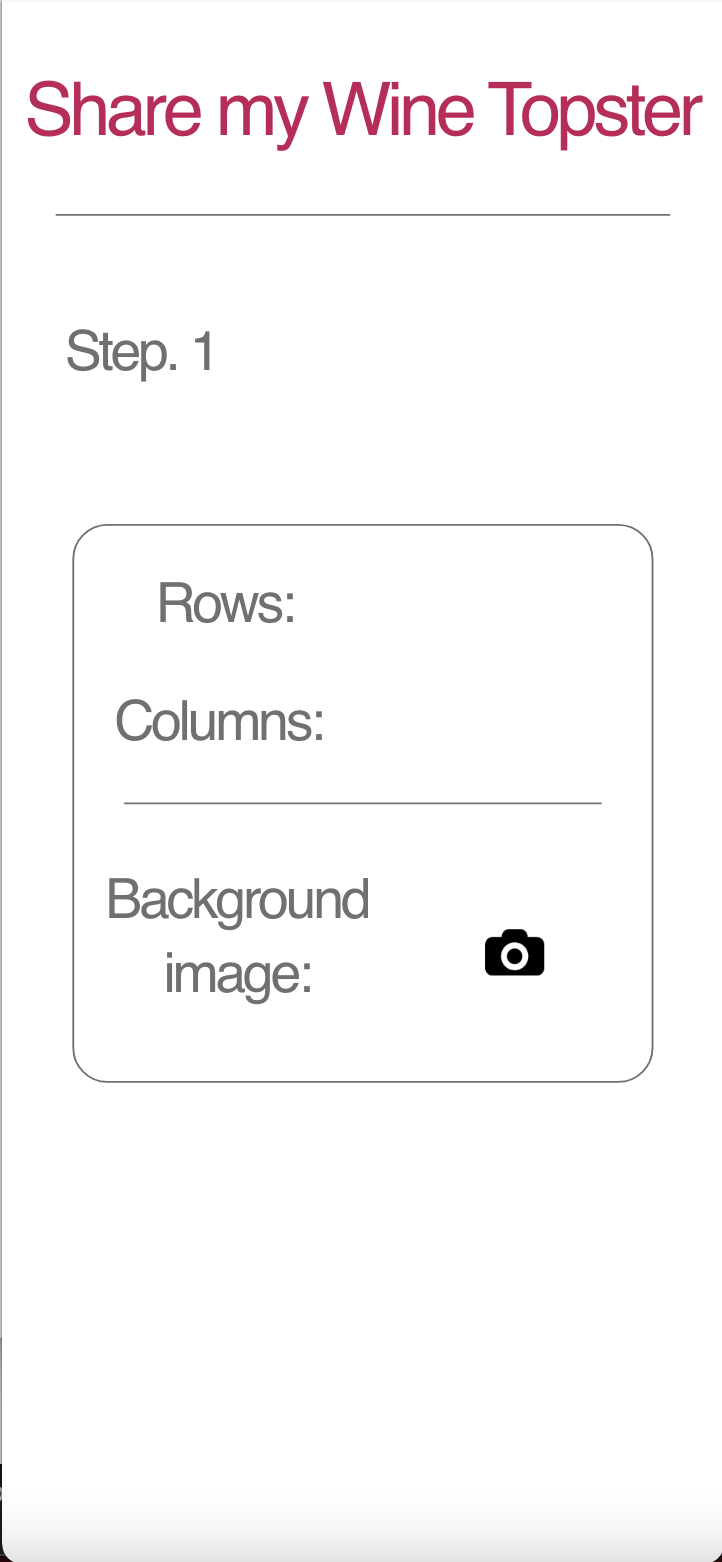
\includegraphics[width=5cm]{top1.png}}
              \item User can set rows \& columns and background image of wine topster.
              \centerline{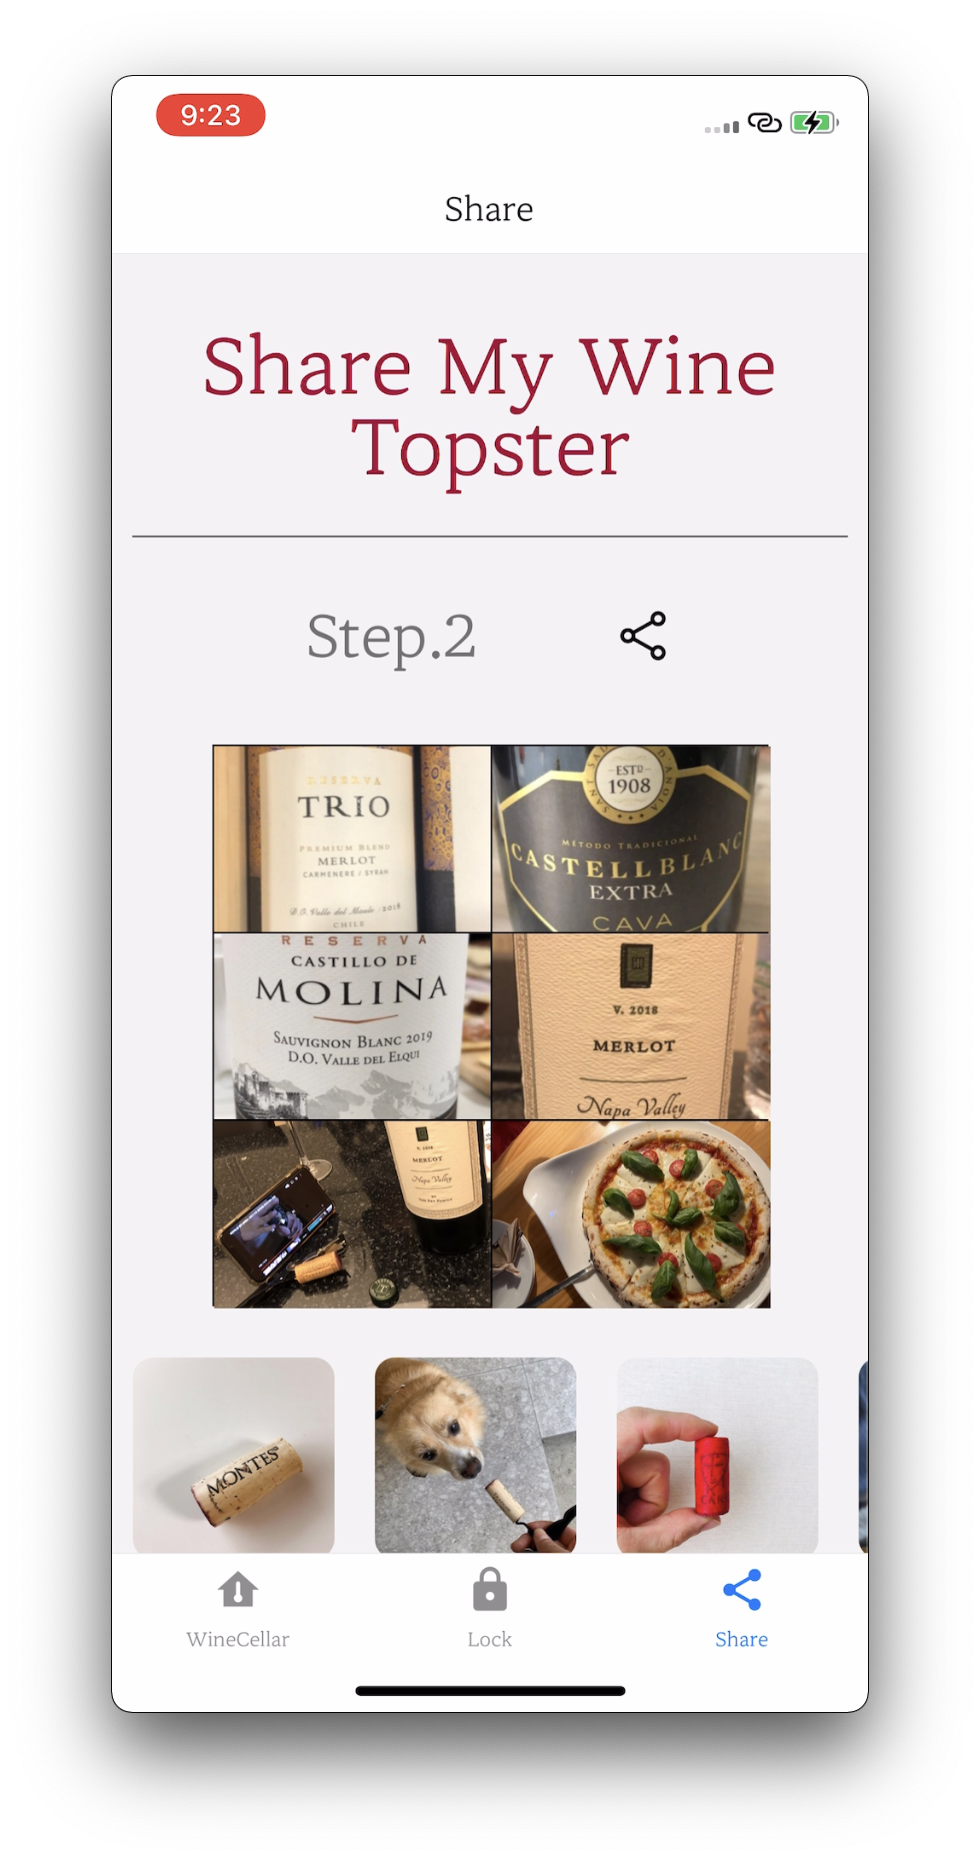
\includegraphics[width=5cm]{top2.png}}
            \item User can make wine topster from setting. User can retrieve image of wine label from database.
        \end{enumerate}
        \end{enumerate}
         \item \textit{\textbf{Wine information}}\\
         \centerline{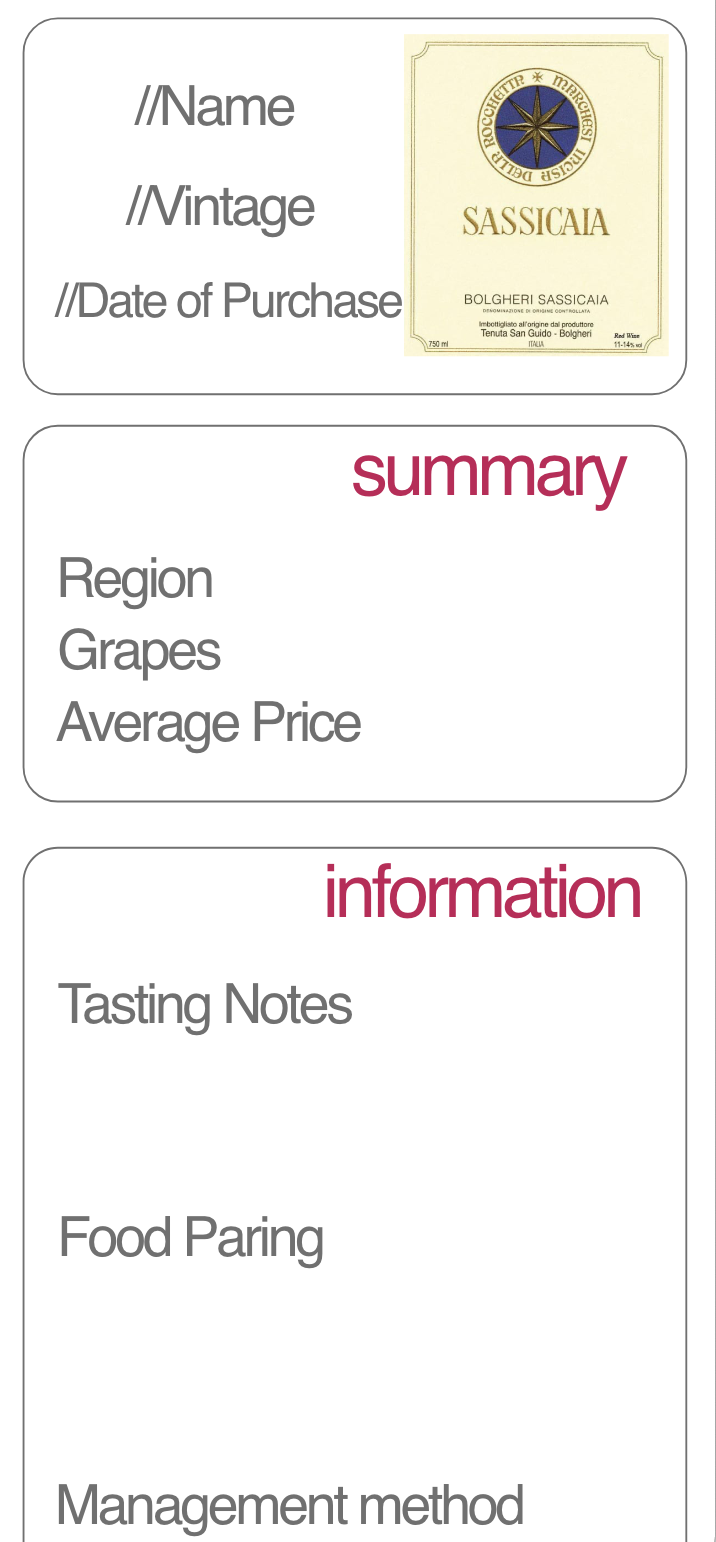
\includegraphics[width=5cm]{wineinfo.png}}
         \centerline{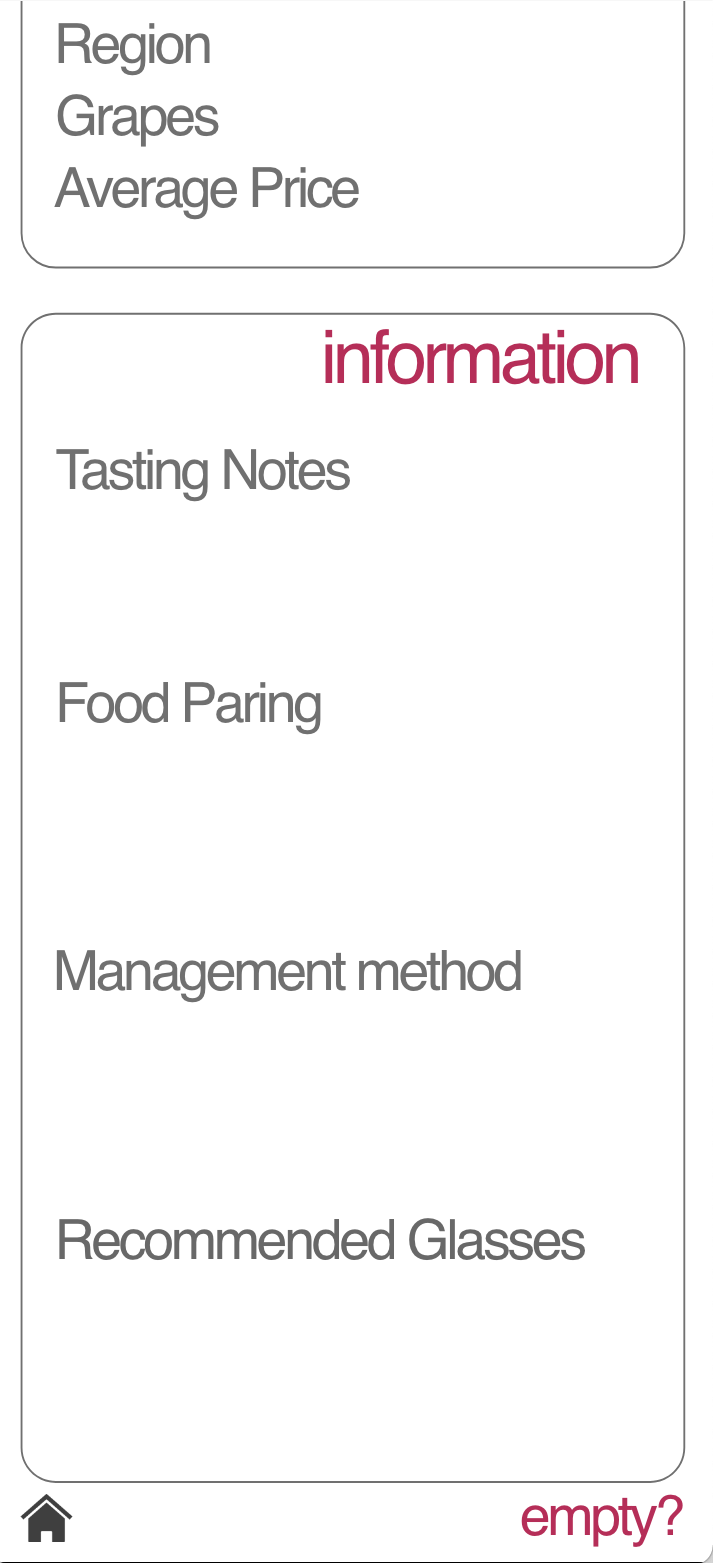
\includegraphics[width=5cm]{wineinfo2.png}}
        All information appears in each container tag. Photo of label, name, wine and date of purchase of wine appear in upper tag. And summary of wine, such as region, grapes and average price of wine appear in middle tag. And information of wine, such as tasting notes, food pairing, management and recommendation glasses appear in lower tag.
    \end{enumerate}
    \item \textit{Settings}\\
    \centerline{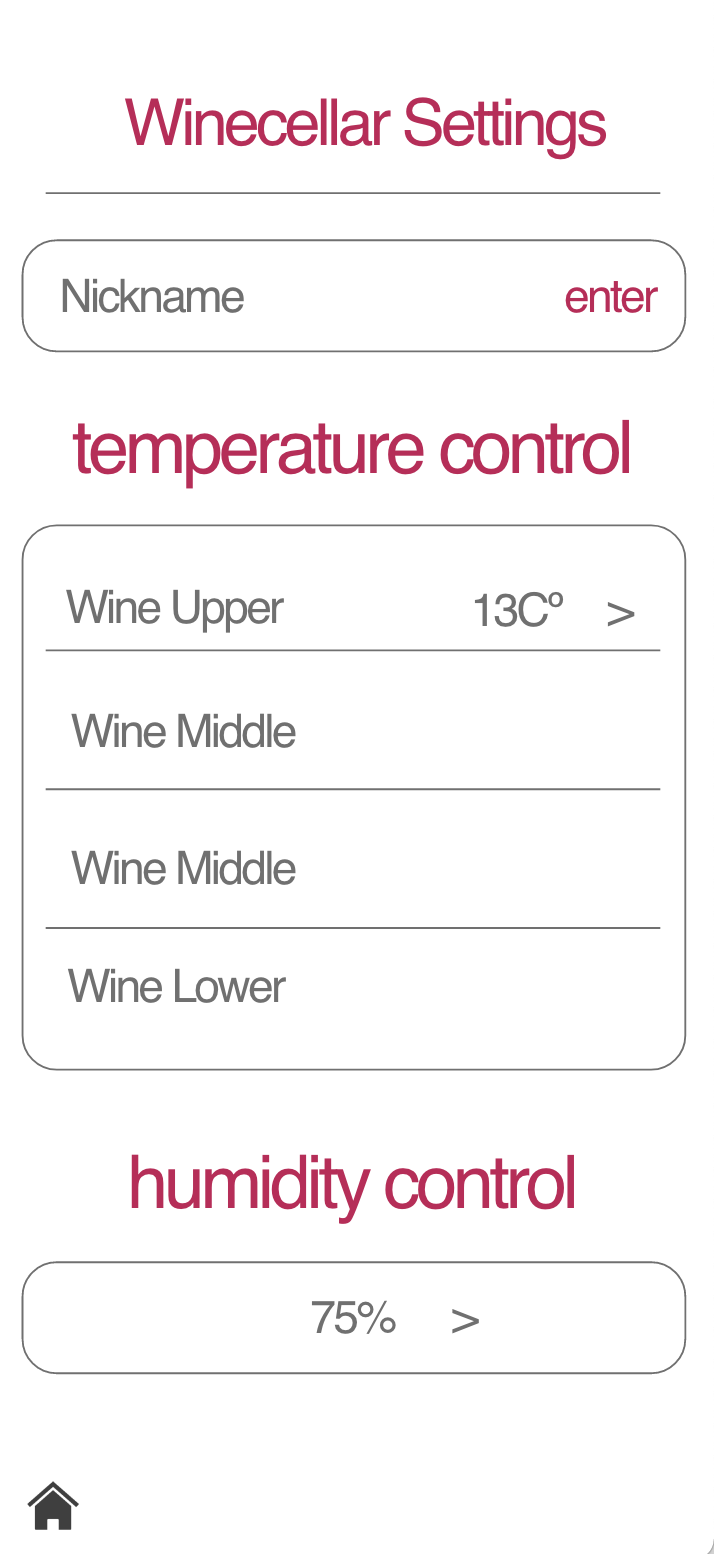
\includegraphics[width=5cm]{setting.png}}
    Settings icon locates next to My Wine Cellar(main page). If user pushes settings icon, user can control wine cellar.
    \begin{enumerate}
        \item \textit{Nickname}\\
        The default name of wine cellar is ‘My Wine cellar–1’. User can change it and generate own nickname. Nickname allows user who has many wine cellars to distinguish one from many wine cellar.
        \item \textit{Temperature control}\\
        A there is difference in appropriate temperature of wine, user can control temperature of each floor of wine cellar.
        \item \textit{Humidity control}\\
        User can control humidity of wine cellar.
        \item \textit{Image of wine label}\\
        When user clicks the image of wine label in main page, user goes to wine information page directly.
    \end{enumerate}
\end{enumerate}
\end{document}